\documentclass[article]{jss}
\usepackage{amsmath,amssymb,enumerate,array,lmodern,thumbpdf}
\shortcites{pomp,raue2009structural,maiwald2016driving,raue2013lessons}

%%\pdfinclusioncopyfonts=1

\DeclareMathOperator*{\argmin}{arg\,min}
\DeclareMathOperator*{\argmax}{arg\,max}

\newcommand{\m}[2]{\textcolor{green}{#1}\textcolor{yellow}{#2}}
\newcommand{\q}[2]{\textcolor{red}{#1}\textcolor{blue}{#2}}

\author{Daniel Kaschek\\University of Freiburg \And
	Wolfgang Mader\\University of Freiburg \AND
	Mirjam Fehling-Kaschek\\University of Freiburg \And
	Marcus Rosenblatt\\University of Freiburg \And
	Jens Timmer\\University of Freiburg}
\Plainauthor{Daniel Kaschek, Wolfgang Mader, Mirjam Fehling-Kaschek, Marcus Rosenblatt, Jens Timmer}

\title{Dynamic Modeling, Parameter Estimation and Uncertainty Analysis in \proglang{R}}
\Plaintitle{Dynamic Modeling, Parameter Estimation and Uncertainty Analysis in R}
\Shorttitle{Dynamic Modeling and Parameter Estimation in \proglang{R}}

\Abstract{
In a wide variety of research fields, dynamic modeling is employed as an instrument to learn and understand complex systems. The differential equations involved in this process are usually non-linear and depend on many parameters whose values determine the characteristics of the emergent system. The inverse problem, i.e., the inference or estimation of parameter values from observed data, is of interest from two points of view. First, the existence point of view, dealing with the question whether the system is able to reproduce the observed dynamics for any parameter values. Second, the identifiability point of view, investigating invariance of the prediction under change of parameter values, as well as the quantification of parameter uncertainty.

In this paper, we present the \proglang{R} package \pkg{dMod} providing a framework for dealing with the inverse problem in dynamic systems modeled by ordinary differential equations. The uniqueness of the approach taken by \pkg{dMod} is to provide and propagate accurate derivatives computed from symbolic expressions wherever possible. This derivative information highly supports the convergence of optimization routines and enhances their numerical stability, a requirement for the applicability of sophisticated uncertainty analysis methods. Computational efficiency is achieved by automatic generation and execution of \proglang{C} code. The framework is object-oriented (\proglang{S3}) and provides a variety of functions to set up ordinary differential equation models, observation functions and parameter transformations for multi-conditional parameter estimation.

The key elements of the framework and the methodology implemented in \pkg{dMod} are highlighted by an application on a three-compartment transporter model.
}

\Keywords{dynamic models, parameter estimation, code generation, maximum likelihood, uncertainty analysis}

\Volume{88}
\Issue{10}
\Month{March}
\Year{2019}
\Submitdate{2016-10-19}
\Acceptdate{2017-12-17}
\DOI{10.18637/jss.v088.i10}

\Address{
  Daniel Kaschek\\
  University of Freiburg\\
  Institute of Physics\\
  Hermann-Herder-Str.~3\\
  79104 Freiburg, Germany\\
  E-mail: \email{daniel.kaschek@gmail.com}
}


\begin{document}

\section{Introduction}

Dynamic systems modeled by ordinary differential equations (ODEs) are found in several research fields, such as physics, biology or finance. In all these fields, models link theoretical concepts and empirical evidence.
Single mechanisms or single processes of a complex system are represented by respective terms in the equations of a dynamic model. Parameter estimation can then identify those processes which are crucial to explaining the observation.
In that sense, parameter estimation can be employed as an instrument to \textit{understand} complex systems. Once the link between observation and model has been established by the estimated parameters, questions about their identifiability arise. The parameter space needs to be explored in order to analyze whether the estimate is unique and to determine confidence bounds.

Although the problem of parameter estimation in non-linear ODE models is highly relevant and at the heart of statistical computing, there are currently not more than four \proglang{R} packages published on the topic on the Comprehensive \proglang{R} Archive Network (CRAN), namely \pkg{FME} \citep{FME}, \pkg{nlmeODE} \citep{nlmeODE}, \pkg{mkin} \citep{mkin} and \pkg{scaRabee} \citep{scaRabee}. All packages have in common that they are built upon the \pkg{deSolve} package \citep{deSolve}. Taking a broader perspective on the topic of dynamic modeling and inference, we find more packages, dealing with, e.g., discrete-time and continuous-time stochastic systems \citep{CollocInfer} or the statistical inference of partially observed Markov processes \citep{pomp}.

The packages \pkg{mkin} and \pkg{FME} support ODEs defined by compiled code while \pkg{mkin} also provides tools to autogenerate the \proglang{C} code and compile it using the \pkg{inline} package \citep{inline}. For model fitting and uncertainty analysis, \pkg{mkin} fully resorts to the functionality of \pkg{FME}.
Concerning model fitting, \pkg{FME} and \pkg{nlmeODE} (with \pkg{nlme} in the background) use deterministic derivative-based optimizers by default, i.e., either Levenberg-Marquardt or Newton methods provided by \code{nls.lm()}, \code{optim()} or \code{nlmimb()}. Although all these optimizers support gradient or Hessian information as input, only the \pkg{nlmeODE} package provides an option to augment the ODE by its sensitivity equations to generate derivates for the residuals. By default, sensitivities are computed by finite differences. Last but not least, the \pkg{scaRabee} package uses the Nelder-Mead optimization algorithm which is derivative-free but generally needs more iterations until convergence compared to derivative-based methods.
In all packages, uncertainty analysis is by default based on the variance-covariance matrix, i.e., non the inverse Hessian matrix of the least squares function. For non-linear models, this method provides a good approximation only if parameters are identifiable and the data is highly informative. If these conditions are not met, more sophisticated methods like, e.g., Markov chain Monte Carlo (MCMC) sampling, implemented in \pkg{FME}, are required.
The strength of \pkg{scaRabee} and especially \pkg{nlmeODE} is multi-conditional fitting. This means that the same model with the same parameters but different forcings to reflect experimental conditions is fitted simultaneously to the condition-specific data sets. In the context of mixed-effects modeling as provided by \pkg{nlmeODE}, parameters can be grouped in fixed effects (parameters are the same in all conditions) and random effects (parameters are different between conditions).

In this paper we present \pkg{dMod}, an \proglang{R} package on dynamic modeling and parameter estimation. 
The package has grown over the past years and reflects many developments and lessons learned from our research projects with time-resolved experimental data from systems biology. They form the basis of the development of \pkg{dMod} and are found as references in the following paragraphs. The aim and core functionality of \pkg{dMod} is summarized in Table~\ref{tab:comparison}, first column. A comparison with the other packages is shown in the remaining columns. 

\begin{table}[t!]
\centering
\begin{tabular}{m{7cm} ccccc}
\hline
& \pkg{dMod} & \pkg{FME} & \pkg{nlmeODE} & \pkg{scaRabee} & \pkg{mkin}\\ \hline
Facilitated set-up of ODE models with automated \proglang{C} code generation for fast simulation of model predictions and model sensitivities & $+$ & $(+)^1$ & $-$ & $-$ & $(+)^1$ \\ \hline
Flexible set-up of general parameter transformations (explicit or implicit) and observation functions, allowing for the implementation of multiple experimental conditions similar to mixed-effects modeling & $+$ & $-$ & $(+)^2$ & $(+)^2$ & $-$ \\ \hline
Parameter estimation based on trust-region optimization of the negative log-likelihood, making use of the sensitivity equations of the dynamic system and of symbolic derivatives of the observation- and parameter transformation functions & $+$ & $-$ & $-$ & $-$ & $-$ \\ \hline
Identifiability and uncertainty analysis based on the profile-likelihood method to determine confidence intervals for parameters and predictions & $+$ & $(-)^3$ & $-$ & $-$ & $-$ \\ \hline
\end{tabular}
\caption{\label{tab:comparison} Overview of the \pkg{dMod} core functionality and comparison with other packages.
1~=~Only~ODE, no sensitivity equations generated.
2 = Mixed-effects modeling allows to define parameters in a condition-specific manner.
3 = Other methods used, e.g., the collinearity method \citep{brun2001practical}.}
\end{table}

The \pkg{dMod} package deals with noise in the observation but not with noise in the dynamics. Therefore, the application of \pkg{dMod} is restricted to systems that are described or can be approximated by a deterministic set of differential equations. 
The core functionality is extended by two symbolic methods implemented in \proglang{Python} and interfaced via the \pkg{rPython} package: identifiability and observability analysis based on Lie-group symmetries \citep{merkt2015higher} and steady-state constraints for parameter estimation \citep{rosenblatt2016customized}.

The implementation of capabilities to generate and propagate derivatives on a compiled-code level distinguishes \pkg{dMod} from other modeling frameworks as discussed above. Most of the standard optimization routines implemented in \proglang{R} need derivative information. However, the computation of derivatives in the context of ODE models holds some pitfalls. The accuracy of sensitivities obtained from finite differences can be insufficient because the step control of the integrator presents an additional source of numeric inaccuracy. Even for numeric methods circumventing this problem, e.g., complex-step derivatives \citep{squire1998using}, the use of sensitivity equations is still beneficial judging from the accuracy vs.~computational cost ratio. See \cite{raue2013lessons} for a comparison of methods.

Another distinguishing feature of \pkg{dMod} is the handling of non-identifiability of parameters, a phenomenon that occurs frequently in the context of parameter estimation in dynamic systems.
In some cases, non-identifiability has structural reasons. The differential equations bear certain symmetries which can or cannot be broken, depending on the structure of the observation. A functional relationship between parameters that leaves the observation invariant is the consequence of the latter. In other cases, the data allows the determination of a unique optimum but other solutions, although worse, cannot be statistically rejected. The \pkg{dMod} package deals with parameter identifiability and parameter uncertainty by the profile-likelihood method \citep{murphy2000profile, raue2009structural, kreutz2013profile}. This method has proven especially useful in the case of non-identifiable parameters where results obtained from both the quadratic approximation by the variance-covariance matrix and MCMC sampling can be misleading \citep{raue2013joining}. Besides parameter uncertainties, the profile likelihood method allows the estimation of prediction uncertainty \citep{kreutz2012likelihood}. It therefore supports the planning of new informative experiments \citep{raue2011addressing} or suggests possible model reductions \citep{maiwald2016driving}.

The key methods implemented in \pkg{dMod} are illustrated in great detail on a dynamic model of bile acid flow. The example is a showcase of how modeling \textit{is} a dynamic process, using the analysis tools implemented in \pkg{dMod} to predict, plan new experiments, combine data from different experiments and include non-linear parameter constraints to improve parameter identifiability. In this way, we demonstrate that dMod is a fully developed, flexible modeling environment, which is not only fast (thanks to compiled code), but also reliable (thanks to symbolic derivatives) and accurate (thanks to advanced statistical methods). 

The paper is organized as follows: Section~\ref{sec:theory} introduces the mathematical set-up of dynamic modeling, symmetries in dynamic systems, parameter estimation by the maximum-likelihood method and the profile likelihood. Section~\ref{sec:implementation} discusses the implementation and design principles behind the \pkg{dMod} software. The functionality of \pkg{dMod} is presented in Section~\ref{sec:example} on the example of bile acid flow in a three-compartment model. Finally, Section~\ref{sec:extensions} discusses the two \proglang{Python} extensions shipped with \pkg{dMod}.

The \pkg{dMod} package is available on the Comprehensive \proglang{R} Archive Network at \url{http://CRAN.R-project.org/package=dMod}. The project is hosted on GitHub at \url{https://github.com/dkaschek/dMod}, where more information about system requirements and installation is available. \pkg{dMod} is licensed under the GPL-3 license. 

\vspace*{-0.3cm}

\section{Theoretical background}
\label{sec:theory}

\subsection{Dynamic models and model sensitivities}
Dynamic models describe systems with states $x$, usually quantifying the involved species, their interaction and evolution over time. %  as e.g. given by chemical reaction networks.
The time evolution of the states is expressed via a set of ODEs, $\dot x = f(x)$. Although constituting quite a special class of dynamic systems, chemical reaction networks formulated by the law of mass action as considered here allow for surprisingly general applications. Typical ODE examples derived from the law of mass action are:
\begin{itemize}
\item $\dot x_A = k_p$, constant production of $x_A$ ($\emptyset \rightarrow A$)
\item $\dot x_C = k_c \,x_A \,x_B = - \dot x_A = - \dot x_B$, complex formation ($A+B \rightarrow C$)
\item $\dot x_C = - k_d \,x_C$, proportional degradation of $x_C$ ($C \rightarrow \emptyset$)\,.
\end{itemize}
A general chemical reaction 
\begin{align}
\nu_1 X_1 + \dots + \nu_n X_n \longrightarrow \nu'_1 X_1 + \dots + \nu'_n X_n
\label{eq:ma_chemical}
\end{align}
for species $X_j$, $j = 1, \dots, n$, and stoichiometric coefficients $\nu_j, \nu'_j\in\mathbb N$ translates into the ODE
\begin{align}
\dot x_j = \underbrace{k_0 \left(\prod x_i^{\nu_i}\right)}_{w_0(x, k_0)} (\nu_j' - \nu_j),
\label{eq:ma}
\end{align}
where $k_0$ is the reaction rate.  When several reactions $1, \dots, r$ are involved, all contributions have to be summed up which can be expressed by the matrix equation
\begin{align}
\dot x = S w(x, k).
\label{eq:Sv}
\end{align}
Here, $S$ denotes the $n\times r$ stoichiometry matrix where each column corresponds to one reaction and the coefficients within one column are the values $\nu'_j - \nu_j$ of the corresponding reaction. The vector $w(x, k)$ denotes the vector of $r$ reaction fluxes where the vectors $x$ and $k$ correspond to states and rate constants, respectively.
Equation~\ref{eq:Sv} also holds for general ODEs that do not follow from mass action kinetics. Moreover the system may be explicitly time-dependent and may contain forcings $u(t)$ which, e.g., describe the external stimulation of the system. A general form of the dynamic model is therefore given by
\begin{align}
\dot x = f(x,k,u,t) = S w(x,k,u,t), \quad\quad \textrm{with }  x(t = 0) = x_0.
\end{align}
The solution $x(t,\theta)$ for a given parameter vector $\theta = (k, x_0)$ is called model prediction. %The parameters $\theta$ contain the rate constants, initial values $x_0$ and additional parameters included in the forcings.
It is generally assumed that the stoichiometry matrix $S$ of the system is known.
Besides the model predition itself, also the sensitivity of the prediction to changes in the parameter values is of interest.
The sensitivities $s_i = \frac{\partial x}{\partial \theta_i}$ satisfy the \textit{sensitivity equations}
\begin{align}
\dot s_i  = \frac{\partial f}{\partial x} s_i + \frac{\partial f}{\partial \theta_i}, \qquad \textrm{with }s_i(t = 0) = \frac{\partial x_0}{\partial \theta_i},
\end{align}
a system of ordinary differential equations that in general depend on the states $x$ and, therefore, need to be solved jointly with the original ODE.

Often, the experimentally observed quantities $y$ do not directly correspond to the species $x$ described by the ODE, but are obtained via an observation function $g: \mathbb{R}^n \rightarrow \mathbb{R}^m$,  \begin{align}
	y = g(x, c)
\label{eq:observation}
\end{align}
with the observation parameters $c$. Examples for observation functions are scaling and offset transformations, $y = c_s \cdot x + c_o$, or the measurement of a superposition of species, $y_i = \sum_j c_j x_j$. The model prediction for the observed states is obtained by evaluating the observation function on the solution of the ODE. Following the chain rule of differentation also the sensitivities of the observed states $\frac{\partial y}{\partial \theta_i} = \frac{\partial g}{\partial x} \frac{\partial x}{\partial\theta_i}  + \frac{\partial g}{\partial \theta_i}$ are obtained. Here, the parameter vector $\theta$ has been augmented by the observation parameters, $\theta = (k, x_0, c)$.

The estimation of the parameters $\theta$ given the observation $y(t)$ is addressed in the next section.


\subsection{Maximum-likelihood method}

Parameter estimation is a common task in statistics. It describes the process of inferring parameter values or parameter ranges of a statistical model based on observed data. Over decades, appropriate estimators have been developed for different problem classes. The principle of maximum likelihood allows to derive an estimator which is especially suited for applications where the distribution of the measurement noise is known. This knowledge about the structure of the noise constitutes additional information that makes the maximum-likelihood estimator (MLE) \textit{efficient}, i.e., from all unbiased estimators the MLE has the lowest variance. Other properties of maximum-likelihood estimation are \textit{consistency}, i.e., the estimated parameter value approaches the true parameter value in the limit of infinite data-sample size, and \textit{asymptotic normality}, i.e., in the limit of infinite data the MLE follows a multivariate normal distribution. See \cite{azzalini1996statistical} for an introduction to likelihood theory.

Maximum-likelihood estimation is based on the maximization of the likelihood function $L(\theta) = \phi(y^D|\theta)$. Here, $\phi$ is the joint probability density for a vector of observations $y$, c.f.~Equation~\ref{eq:observation}, evaluated at the point $y = y^D$, the vector of data points. The distribution $\phi$ depends parametrically on model parameters $\theta$. The maximum-likelihood estimator $\hat\theta$ is defined as
\begin{align*}
\hat \theta := \argmax_{\theta} L(\theta),
\end{align*}
meaning that $\hat\theta$ is an extremum estimator. Depending on the model class and the probability distribution $\phi$, maximization of the likelihood can be a challenge beyond the scope of analytical methods. Numerical optimization methods help to solve the maximization problem in practical applications.

The easiest and one of the most frequent situations is when $\phi$ follows a normal distribution, $\phi\sim\mathcal N(y(\theta), \Sigma)$. When measurements are statistically independent, the variance-covariance matrix $\Sigma = {\rm diag}(\sigma_1^2, \dots, \sigma_N^2)$ is diagonal and $\phi$ factorizes. The likelihood function reads 
\begin{align}
	L(\theta) &= \prod_{i = 1}^N \frac{1}{\sqrt{2\pi\sigma_i^2}} e^{-\frac{(y_i(\theta)-y_i^D)^2}{2\sigma_i^2}} .
\label{eq:likelihood}
\end{align}
Taking twice the negative logarithm, Equation~\ref{eq:likelihood} turns into
\begin{align}
	l(\theta) = -2\log L(\theta) &= \sum_i \left[\left(\frac{y_i(\theta) - y_i^D}{\sigma_i}\right)^2 + \log(2\pi\sigma_i^2)\right],
\label{eq:nll}
\end{align}
thus converting the maximization of $L(\theta)$ to a minimization of $l(\theta)$.
Assuming that the data uncertainties $\sigma_i$ are known, Equation~\ref{eq:nll} is the weighted least-squares function shifted by a constant. For unknown $\sigma_i$, Equation~\ref{eq:nll} can be optimized with respect to $\theta$ and $\sigma$ jointly, yielding the MLE $\hat\theta^{\prime} = (\hat\theta, \hat\sigma)$. 

\subsection{Non-linear optimization}

Numerical optimization is a diverse field with as many algorithms as there are optimization problems around. The \pkg{dMod} package supports derivative-based methods, and in particular the Newton method.

Optimization by the Newton method attempts to iteratively find the root of the gradient $\nabla l (\theta)$ by the recursion
\begin{align}
\theta^{(n+1)} = \theta^{(n)} - Hl(\theta)^{-1}\nabla l(\theta),
\label{eq:newton}
\end{align}
where $Hl(\theta)$ denotes the Hessian, i.e., the matrix of second derivatives of $l(\theta)$. The fact that for normally distributed noise the log-likelihood is a least squares function, has a big advantage: gradient and (approximate) Hessian can be computed from first-order derivatives  \citep{press1996numerical}. Since the second-order contributions to the Hessian can be neglected, gradient and Hessian read
\begin{align}
\nabla l(\theta) = 2 r(\theta) J(\theta) \quad\quad Hl(\theta) \approx 2 J(\theta)^T J(\theta),
\label{eq:derivatives}
\end{align}
with the weighted residual vector $r_i(\theta) = \frac{y_i(\theta) - y_i^D}{\sigma_i}$ and its first derivative, the Jacobian matrix
\begin{align}
	J_{ij}(\theta) = \frac{\partial r_i}{\partial \theta_j}(\theta) = \frac{1}{\sigma_i} \frac{\partial y_i}{\partial \theta_j}(\theta). \label{eq:jacobian}
\end{align}
As indicated by eqs.~\eqref{eq:derivatives}-\eqref{eq:jacobian},  first order model sensitivities $\frac{\partial y_i}{\partial\theta_j}$ are sufficient to compute gradient and Hessian in good approximation.

The Newton recursion, Equation~\ref{eq:newton}, converges in one iteration if $l(\theta)$ is a quadratic form. However, $l(\theta)$ is only quadratic if the model $y(\theta)$ is linear in $\theta$ which is usually not the case for ODE models. On the other hand, each smooth function, no matter if quadratic or not, can be approximated by a quadratic function based on its Taylor series.
Thus, $l(\theta)$ can be approximated by a quadratic function in at least a small region around $\theta$. The idea of trust-region optimization is to confine a Newton step to a region, the \textit{trust region}, where the quadratic approximation holds \citep{wright1999numerical}.
In each iteration, the trust-region radius is adjusted and the optimization problem restricted to the trust region is solved. For parameter estimation in ODE models this has the additional advantage that parameter changes are constricted and optimization steps into parameter regions where the ODE cannot be numerically solved any more  become less frequent. This makes trust-region optimization the method of choice for \pkg{dMod}.



% Hier auf Maximum-Likelihood vs. least-squares function eingehen.

\subsection{Parameter uncertainty analysis}

Parameter estimates $\hat \theta$  are obtained by non-linear optimization of the log-likelihood function $l(\theta)$. Although being a function of the parameters,  the log-likelihood depends on the data, too. Consequently, ``equivalent'' random realizations of the data would lead to different parameter estimates $\hat\theta$. Given $\hat\theta$ for one random realization of the data, the question is, at which significance level we can reject other parameters $\theta$. This leads to the related question of parameter convidence intervals.

A useful tool to derive confidence intervals beyond the scope of Fisher Information Matrix is the profile likelihood \citep{venzon1988method, murphy2000profile}. Consider a parameter of interest, $\theta_i$, being one of the parameters in the vector $\theta$. Furthermore, let $c_{\tau}(\theta) = \theta_i - \tau = 0$ be a parameter constraint.
Then, extending the likelihood with the constraint via a Lagrange multiplier $\lambda$ yields
\begin{align}
\begin{aligned}
{\rm pl}_i:\quad \mathbb R & \longrightarrow \mathbb R\\
\tau & \longmapsto \min_{(\theta, \lambda)} \big[ l(\theta) + \lambda c_{\tau}(\theta) \big]
\end{aligned}
\label{eq:pl}
\end{align}
which is called the profile likelihood of the $i^{\;\rm th}$ parameter. The path $\tau \mapsto (\hat\theta_{\tau}, \hat\lambda_{\tau})$ along the minimizing parameters is called the profile likelihood path. Hence, the profile likelihood ${\rm pl}_i$ returns the minimal log-likelihood under the constraint $\theta_i \stackrel{!}{=} \tau$. By construction, the inequality $D_i := {\rm pl}_i(\tau) - {\rm pl}_i(\hat \theta_i) \geq 0$ holds for all $\tau$, assuming equality at least for $\tau = \hat\theta_i$. Interpreting the unconstrained model as the null model, which we assume to be true, and that with $\theta_i$ fixed to $\tau$ as the alternative model, the value $D$ is twice the log of the likelihood-ratio between those. Hence, a likelihood-ratio test can be performed to accept or reject the alternative model at a given confidence level. To compute the corresponding threshold, we assume a sufficiently large sample size to apply Wilks' theorem according to which the thresholds are the quantiles of the $\chi^2$ distribution with one degree of freedom. Consequently, the $68\%/90\%/95\%$-confidence intervals of $\theta_i$ are those values of $\tau$ for which $D_i(\tau) \leq 1$, $2.71$ and $3.84$, respectively.

The reason to formulate the profile likelihood by Lagrangian multipliers is that we can directly use Equation~\ref{eq:pl} to derive the profile likelihood path $(\hat \theta_{\tau}, \hat\lambda_{\tau})$ with respect to $\tau$:
\begin{align}
\frac{\rm d}{{\rm d} \tau}
\begin{pmatrix}
\hat\theta_{\tau} \\ \hat\lambda_{\tau}
\end{pmatrix} =
\begin{pmatrix}
Hl(\hat\theta_{\tau}) & \nabla c_{\tau}(\hat \theta_{\tau})\\
\nabla c_{\tau}(\hat\theta_{\tau})^T & 0
\end{pmatrix}^{-1}
\begin{pmatrix}
0 \\ 1
\end{pmatrix}.
\label{eq:path}
\end{align}
Equation~\ref{eq:path} forms the basis of what is implemented in \pkg{dMod} for computing the profile likelihood.

The profile likelihood approach can be applied to compute confidence intervals for model predictions, too, see \cite{kreutz2012likelihood, hass2016fast}.

\vspace*{-0.3cm}

\section{Implementation and design principles}
\label{sec:implementation}

The guiding idea behind the implementation of \pkg{dMod} is to provide a class structure for models, predictions, observations and parameter transformations that allows a flexible combination of many experimental conditions in one objective function to fit models to data. This flexibility is achieved by two concepts: (1) concatenation of functions by the \code{"*"} operator and (2) stacking of functions representing different conditions by the \code{"+"} operator. The handling and propagation of derivatives is part of the classes and happens in the background. Methods for the generic \code{print()}, \code{plot()} and \code{summary()} functions are implemented for most outputs.

\vspace*{-0.3cm}

\subsection{Model formulation}

A system of ODEs $\dot x = f(x, p, u, t)$ is represented by a named \code{character} vector of symbolic expressions, the right-hand side of the ODE, involving symbols for the states $x$, the parameters $p$, the forcings $u$ and the keyword \code{time} for $t$. The names of the vector are the state names. The class provided by \pkg{dMod} for such objects is the \code{eqnvec} class which checks whether the character can be parsed and thus, can be interpreted as an equation.

\pkg{dMod} provides several ways to define the differential equations. An \code{eqnvec} of equations can be explicitly formulated, analogously to a \code{c()} command. Especially for chemical reactions it can be tedious to keep track of all gain and loss terms. Therefore, \pkg{dMod} provides also the \code{eqnlist} class which encodes the ODE by a list of (1) state names, (2) rate expressions, (3) compartment volumes and (4) the stoichiometric matrix. Each reaction flux, c.f.~Equation~\ref{eq:Sv}, occurs only once and the gain and loss is represented by the coefficients in the stoichiometric matrix. \pkg{dMod} supports the read-in of a csv file with the stoichiometric matrix and rate expressions and provides a function \code{addReaction()} to construct an \code{eqnlist} object step-by-step or add further reactions to an already existing \code{eqnlist}. An \code{eqnlist} is converted to (differential) equations, i.e., an \code{eqnvec}, by \code{as.eqnvec()}. The conversion does all the bookkeeping of gain and loss terms and volume ratios due to compartment transitions.

\pkg{dMod} makes use of derivatives wherever possible. It is one of the core functionalities of the \pkg{cOde} package \citep{cOde} upon which \pkg{dMod} is based to augment a system of ODEs by its sensitivity equations. If $r$ parameters are involved and the system consists of $n$ states, the number of equations grows as quick as $n^2 + nr$. Solving the equations can be considerably accelerated by utilizing compiled code. \pkg{dMod} provides the \code{odemodel} class. An object of class \code{odemodel} is generated from an \code{eqnlist} or \code{eqnvec}. In the background, \proglang{C} code for the ODE and the combined system of ODE and sensitivity equations is generated, written to the working directory and compiled. The \code{odemodel} object keeps track of the shared objects. It is the basis of a prediction function $x(t, p)$ generated by the \code{Xs()} command.

\subsection{Prediction functions}

\pkg{dMod} seeks to stay close to the mathematical formulation, i.e., \code{x <- Xs(myodemodel)} will indeed return an \proglang{R} function, an object of class \code{prdfn}, which expects arguments \code{times} and \code{pars} and turns them into a model prediction. The letter \code{"s"} in \code{"Xs"} refers to sensitivities, i.e., the solution $x(t)$ is returned, the sensitivities $\frac{\partial x}{\partial p}(t)$ are returned, too.

Besides parameters, the prediction might also depend on forcings $u(t)$ and sudden events, e.g., setting states to 0 at a predefined point in time. Since forcings and events are by default fixed, they are defined together with the  prediction function, \code{x <- Xs(odemodel, forcings = myforcings, events = myevents)}. The definitions of both, forcings and events, are compatible with the way they are defined in \pkg{deSolve}.

\subsection{Observation functions}


An observation function is a function $g(x, p_{\rm obs}, t)$ that evaluates the solution $x(t)$ together with additional (observation) parameters $p_{\rm obs}$. The function can explicitly depend on time~$t$. Similar to the ODE case, an observation function can be expressed as a character vector with names corresponding to the names of the observables and equations involving symbols for the states, parameters and the keyword \code{time}. An observation function is defined as an \code{eqnvec} and turned into an \proglang{R} function via \code{Y()}.

It is one of the fundamental concepts of \pkg{dMod} to allow concatenation of functions via the \code{"*"} operator. The mathematical formulation $y = g\circ x$, i.e., $y(t, p) = (g\circ x)(t, p):= g(x(t, p), p, t)$ becomes \code{y = g * x} in \proglang{R}. To obtain derivatives $\frac{\partial y}{\partial p}$, the chain rule is applied: $\frac{\partial y}{\partial p} = \frac{\partial g}{\partial x}\frac{\partial x}{\partial p} + \frac{\partial g}{\partial p}$. This means that \code{Y()} needs to be informed which symbols are states and parameters to generate the corresponding expressions $\frac{\partial g}{\partial x}$ and $\frac{\partial g}{\partial p}$. The observation function \code{g} takes care of computing theses derivatives from the symbolic expressions and doing the matrix multiplication with the sensitivities $\frac{\partial x}{\partial p}$ from the prediction function. Evaluation of symbolic expressions can become inefficient in \proglang{R}. Therefore, the observation function is usually translated into a \proglang{C} code and compiled.

When observation- and prediction functions are concatenated, the result is a prediction function, e.g., \code{y = g * x} is the \proglang{R} function computing values $y(t)$ from the arguments \code{times} and \code{pars} via evaluation of the ODE and subsequent evaluation of the observation function. Two observation functions can be concatenated, too, again yielding an observation function.

\subsection{Parameter transformations}

Parameter transformations are the key element of \pkg{dMod} to formulate different kinds of constraints and allow the combination of several experimental/modeling conditions in one parameter vector.

In principle, a parameter transformation $p = \Phi(\theta)$ is a (differentiable) function connecting \textbf{inner} parameters $p$ with \textbf{outer} parameters $\theta$. The rationale behind the distinction of inner and outer parameters is that the vector $p$ usually desribes those parameters defined in the model equations. The outer parameters $\theta$ refer to a convenient parameterization by which the model parameters are computed. Examples are a log-transform of the inner parameters, $\theta = \log(p) \Leftrightarrow p = \Phi(\theta) = e^{\theta}$, or parameter constraints like $(p_1, p_2) = (\theta_1, \theta_1 + \theta_2)$.

An \proglang{R} function of class \code{parfn} is produced by the \code{P()} command. Transformations can either be formulated explicitly or implicitly. In the explicit case, the function $p = \Phi(\theta)$ corresponds to an \code{eqnvec} whose names are the names of the inner parameters and entries are equations with symbols for the outer parameters. An implicit transformation has the form $f\big(p = \Phi(\theta), \theta\big) = 0$. In this case, $f$ is expressed by an \code{eqnvec} with equations containing symbols for $p$ and $\theta$ and the names of the \code{eqnvec} are the symbols for $p$.

Similar to prediction- and observation functions, parameter functions not only return parameter values but the Jacobian of the transformation, too. Exploiting the chain rule, the derivatives are propagated, allowing to define \code{y = g * x * p} which is a function returning $y(t, \theta)$ and $\frac{\partial y}{\partial \theta}(t)$, i.e., \code{g * x * p} is a prediction function.

Let \code{g}, \code{x}, \code{p1} and \code{p2} be an observation-, a prediction- and two parameter transformation functions. Then \code{p1 * p2} is a parameter transformation function, \code{x * p1} is a prediction function and \code{g * p1} is an observation function.

\subsection{Multi-conditional prediction}

A set of parameter values, forcings and events captures a certain condition in which we find the modeled system. Manipulating the system, single model parameters, forcings or events need to be changed to account for the manipulation. It is a typical approach in systems inference to systematically perturb small parts of a modeled system to reveal information about the processes.

The aim of \pkg{dMod} is to allow for ``simultaneous'' predictions under several conditions and compare these predictions to the corresponding experimental data sets to estimate model parameters.
Different experimental conditions are typically expressed by the fact that some parameters are different between conditions whereas others are common to all conditions. This situation occurs, e.g., if perturbation experiments are performed, affecting only few parts of a system.
%The full information contained in several perturbation experiments is only used if the multi-conditional model prediction is set up in a way that all model parameters not being changed from condition to condition correspond to exactly one parameter. On the other hand, parameters which are systematically perturbed correspond to different parameters.
Mathematically speaking, we want to construct a parameter transformation
\begin{equation}
\begin{aligned}
\Phi:\quad \mathbb R^p & \longrightarrow  \bigoplus_{i = 1}^n \mathbb R^q \\
\theta & \longmapsto  \left(\Phi_1(\theta), \dots, \Phi_n(\theta)\right)
\end{aligned}
\label{eq:partrafo}
\end{equation}
where $i = 1, \dots, n$ corresponds to the different conditions. If all parameters are shared throughout all conditions, then $p = q$. If, however, all parameters are distinct, then $p = n\cdot q$. Perturbation experiments correspond to a situation where $p\gtrsim q$.

The \pkg{dMod} package allows to define transformations $\Phi$, see Equation~\ref{eq:partrafo}, by the \code{"+"} operator:\footnote{We chose the \code{"+"} sign in analogy to the $\oplus$ formulation used for the direct sum of vector spaces in Equation~\ref{eq:partrafo}.}
\begin{verbatim}
  p <- P(eqnvec1, condition = "one") + P(eqnvec2, condition = "two")
\end{verbatim}
All symbols from \code{eqnvec1} and \code{eqnvec2} are collected and their union constitutes the symbols of $\theta$. The evaluation \code{p(theta)} returns a list of length $n$ (in the example $n = 2$) with inner parameters. The \code{"+"} operator can be applied consecutively to add conditions.

Prediction- and observation functions are generalized to multiple conditions by the \code{"+"} operator, too. Mathematically speaking, they become
\begin{align*}
\begin{aligned}
x: &  & \mathbb R \times \bigoplus_{i = 1}^n \mathbb R^q & \longrightarrow  \bigoplus_{i = 1}^n \mathbb R^m \\
 & & (t, p_1, \dots, p_n) & \longmapsto (x_1(t, p_1), \dots, x_n(t, p_n)) \\
g: &  & \bigoplus_{i = 1}^n \mathbb R^m \times \bigoplus_{i = 1}^n \mathbb R^q\times \mathbb R& \longrightarrow  \bigoplus_{i = 1}^n \mathbb R^s \\
& & (x_1(t), \dots, x_n(t), p_1, \dots, p_n, t) & \longmapsto (g_1(x_1(t), p_1, t), \dots, g_n(x_n(t, p_n), p_n, t)).
\end{aligned}
\label{}
\end{align*}
In words, if prediction- or observation functions are defined for different conditions then they expect condition-specific inputs which are evaluated by the matching functions. Examples for condition-specific prediction functions typically involve different forcings or events. Observation functions can, e.g., differ between different measurement techniques. In all these cases, the different prediction functions $x_1, \dots, x_n$ or observation functions $g_1, \dots, g_n$ are defined, referencing the condition, and combined by the \code{"+"} operator analogously to \code{p}.
% Aufruf der Funktionen mit subset von conditions

All commands, \code{P()}, \code{Xs()}, \code{Y()}, etc.~can be executed with \code{condition = NULL}. In that case, the corresponding returned function is generic and, if called for different conditions, the same identical function is evaluated with the condition-specific input. The other way round, if a function, say, \code{x} is defined for several conditions, its prediction can be evaluated only for a subset of conditions by \code{x(times, pars, conditions = myconditions)}.

\subsection{The data structure}

In \pkg{dMod} different experimental conditions are handled by lists. Parameter transformations, prediction- and observation functions stacked by the \code{"+"} operator return list objects. On the other hand, \code{data.frame}s as they are used for linear modeling, mixed-effects modeling or plotting with \pkg{ggplot2} are highly convenient to organize the data.
The class \code{datalist} provides the interface between \pkg{dMod}'s list structures and \code{data.frame} objects.
%For the sake of computational efficiency, we keep the list structure of predictions and implement a class \code{datalist} to adapt the \code{data.frame} objects.
A \code{datalist} is a list of data frames with identical structure: observable names, time points, measured values and measurement uncertainty.

Objects of class \code{datalist} are usually generated by the \code{as.datalist()} command from a \code{data.frame}. The factor variables in the data frame to be used as generators for the unique condition names can be passed by the \code{split.by} argument. The resulting list of data frames has an additional attribute \code{"condition.grid"}, a translation table between the condition names and the original factor variables which can be used for specification of parameter transformations or augmentation of predictions by descriptive columns.


\subsection{Objective function}


The aim of \pkg{dMod} is parameter estimation. The objective function to be minimized for this purpose is twice the negative log-likelihood derived from the normal distribution, see Equation~\ref{eq:nll}. The objective function is produced by the command \code{normL2(data, prdfn)} where \code{data} is a \code{datalist} object and \code{prdfn} is a prediction function. By default, it is expected that the datalist contains non-zero measurment uncertainty values in the \code{sigma} column corresponding to the $\sigma_i$ in Equation~\ref{eq:nll}. However, it is also possible to use  Equation~\ref{eq:nll} to estimate $\sigma$. To this end, an error model needs to be defined as an \code{eqvec} object. The names are expected to be a subset of the obervable names and the equations define the expected $\sigma$ of the observable as a function of error model parameters and the observables themselves. The \code{eqnvec} object is translated into an ``observation function'' by the \code{Y()} command. Finally, the objective function is generated by \code{normL2(data, prdfn, errfn)} with the datalist and prediction function as before and an object \code{errfn} of class \code{prdfn} being the error model function.

The objective function is the final link connecting the chain of parameter transformations, prediction- and observation functions to observations. It collects all derivative information and besides the objective value it also computes gradient and Hessian. The standard optimizer employed within \pkg{dMod} is the \code{trust()} optimizer from the \pkg{trust} package.

Objective functions can be added by the \code{"+"} operator, meaning the objective values, gradients and Hessians are accumulated by summation. Besides the standard function \code{normL2()}, \pkg{dMod} provides several other functions returning objective functions, e.g., \code{constraintL2()} or \code{datapointL2()}. They allow to define quadratic parameter priors or treat data points as parameters, respectively, as shown in Section~\ref{sec:example}. Thus, a typical objective function used for parameter estimation could be
\begin{verbatim}
  obj <- normL2(data, g * x * (p1 + p2 + p3)) + constraintL2(mu, sigma)
\end{verbatim}


\section{Three-compartment model of bile acid transport}
\label{sec:example}

The following model is a simplified dynamic model on bile acid transport published by \cite{kaschek2017dynamic}. Bile acids are produced in the liver. They are necessary for the digestion of fat and oil. In the liver, bile acids are taken up in hepatocytes (liver cells) by specific transporter molecules. Clearance occurs either via canalicular or sinusoidal export, i.e., export to the bile transportation system of bile canaliculi or the intercellular space.

To study bile clearance, experiments with hepatocytes or hepatocyte-derived cell lines are performed \textit{in-vitro}. Cells in a Petri dish stick together to a monolayer of cells, forming bile canaliculi in between cells. They adhere to the dish and are surrounded by a buffer providing the cells with nutrients. A radioactive label allows to measure the bile acid \textit{taurocholic acid} (TCA).

For the mathematical description of bile flow, a three-compartment differential equation model is used. TCA is pipetted into the buffer compartment (\code{TCA_buffer}) from where it is transported into the cells (\code{TCA_cell}). Intracellular TCA is exported back to the buffer or the canalicular compartment (\code{TCA_cana}). Finally, canalicular TCA flows back into the buffer compartment. 

In the following sections, the bile acid example will be used to illustrate key elements of ODE modeling and how they are implemented using \pkg{dMod}. We will start with the implementation of the model itself and show simulation results for the model and model sensitivities. Next, we will introduce the observation function based on radioactive labeling of TCA and will use the model to simulate experimental data. The data will be fitted by the model several times following a multi-start strategy. Parameter identifiability is discussed based on the profile-likelihood method. Finally, different ways to include steady-state constraints in the parameter estimation are discussed and the prediction uncertainty will be assessed.


\subsection{Simulation and prediction}
These processes involved in bile acid transport give rise to the differential equations and corresponding flowchart presented in Figure~\ref{fig:flowchart}. 
\begin{figure}[t!]
\centering
\begin{minipage}{0.55\textwidth}
\textbf{A}
\begin{equation*}
\begin{aligned}
\frac{\texttt d}{ \texttt{dt} } \verb!TCA_buffer! &\texttt{ = } \verb!-import * TCA_buffer!\\
& \quad \verb! + export_sinus * TCA_cell!\\
& \quad \verb! + reflux * TCA_cana!\\
\frac{\texttt d}{ \texttt{dt}} \verb!TCA_cana! &\texttt{ = } \verb!export_cana * TCA_cell!\\
& \quad \verb! - reflux * TCA_cana!\\
\frac{\texttt d}{ \texttt{dt}} \verb!TCA_cell! &\texttt{ = } \verb!import * TCA_buffer!\\
& \quad \verb! - export_sinus * TCA_cell!\\
&\quad \verb! - export_cana * TCA_cell!.
\end{aligned}
\end{equation*}
\end{minipage}
\begin{minipage}{0.44\textwidth}
\textbf{B}\\
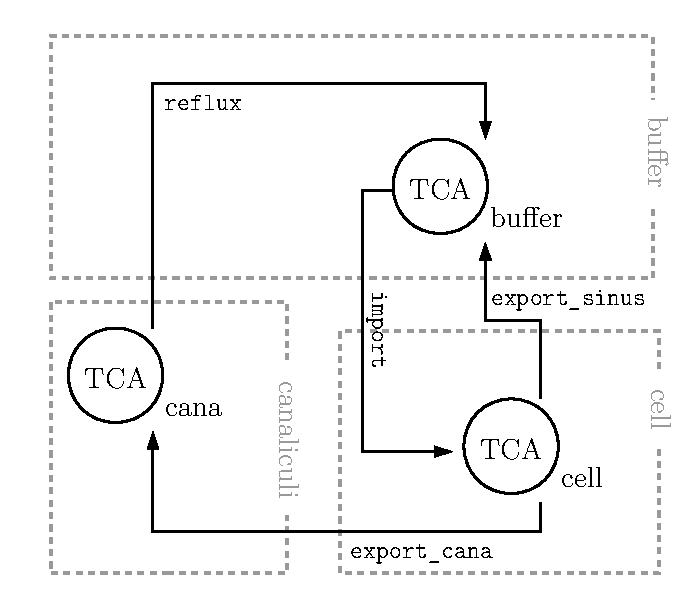
\includegraphics[width = \textwidth]{Figures/flowchart}
\end{minipage}
\caption{Differential equations and flowchart of the reaction network. Taurocholic acid,  TCA, is transported between three compartments by four different processes. (A) Assuming mass-action kinetics, the three dynamic states satisfy a set of coupled differential equations. (B) The equations are visualized in a flowchart. }
\label{fig:flowchart}
\end{figure}
Each transportation process is modeled by mass-action kinetics. A possible implementation in \pkg{dMod} is:
\begin{CodeChunk}
\begin{CodeInput}
R> reactions <- NULL
R> reactions <- addReaction(reactions, "TCA_buffer", "TCA_cell",
+    rate = "import*TCA_buffer", description = "Uptake")
R> reactions <- addReaction(reactions, "TCA_cell", "TCA_buffer",
+    rate = "export_sinus*TCA_cell", description = "Sinusoidal export")
R> reactions <- addReaction(reactions, "TCA_cell", "TCA_cana",
+    rate = "export_cana*TCA_cell", description = "Canalicular export")
R> reactions <- addReaction(reactions, "TCA_cana", "TCA_buffer",
+   rate = "reflux*TCA_cana", description = "Reflux into the buffer")
\end{CodeInput}
\end{CodeChunk}
The reaction list is translated into an ODE model object:
\begin{CodeChunk}
\begin{CodeInput}
R> mymodel <- odemodel(reactions, modelname = "bamodel")
\end{CodeInput}
\end{CodeChunk}
Finally, the prediction function is generated:
\begin{CodeChunk}
\begin{CodeInput}
R> x <- Xs(mymodel, condition = NULL)
\end{CodeInput}
\end{CodeChunk}
The reactions are collected in an \code{eqnlist} object. The \code{odemodel()} command composes the single reactions to an ODE system and auto-generates the \proglang{C} code which is used by the \pkg{deSolve} package to evaluate the ODE. Prediction functions are generated by the \code{Xs()} command. The usage of the prediction function is illustrated by the following code chunk. Time points are defined between 0 and 50, numeric values are assigned to all model parameters. Note that the first three parameters correspond to initial state values.
\begin{CodeChunk}
\begin{CodeInput}
R> times <- seq(0, 50, 0.1)
R> pars <- c(TCA_buffer = 1, TCA_cell = 0, TCA_cana = 0, import = 0.2,
+    export_sinus = 0.2, export_cana = 0.04, reflux = 0.1)
\end{CodeInput}
\end{CodeChunk}
Finally the prediction function is called and both, the prediction and the sensitivities, are plotted, shown in Figure~\ref{fig:prediction}.
\begin{CodeChunk}
\begin{CodeInput}
R> out <- x(times, pars)
R> plot(out)
R> outSens <- getDerivs(x(times, pars[4:7], fixed = pars[1:3]))
R> plot(outSens)
\end{CodeInput}
\end{CodeChunk}
%
\begin{figure}[t!]
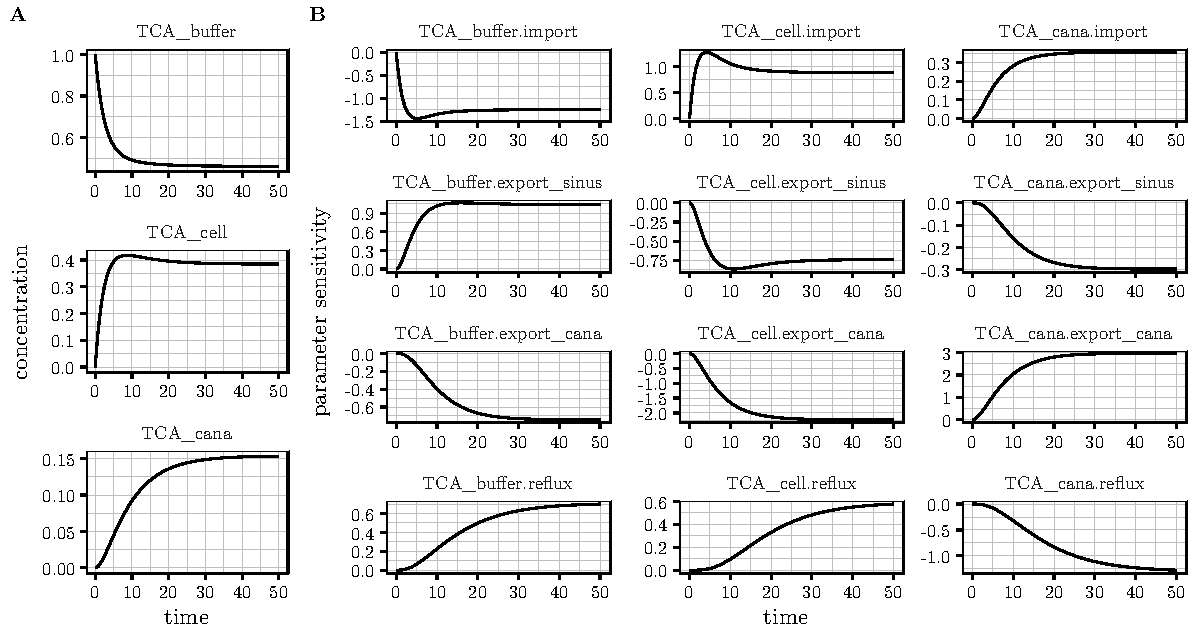
\includegraphics[width = \textwidth]{Figures/figure1}
\caption{Output of the prediction function. (A) Prediction of the TCA states. (B) Sensitivities of the three TCA states for the rate parameters only.\label{fig:prediction}}
\end{figure}
%
Figure~\ref{fig:prediction}A shows the uptake of \code{TCA_buffer} in the cell and canaliculi, saturating around $t = 50$. The prediction parametrically depends on initial values and rate parameters. Figure~\ref{fig:prediction}B shows the model sensitivities $\frac{\partial x}{\partial p}$ for the rate parameters.

\subsection{Observation function and simulated data}
In experiments, the three dynamic states, \code{TCA_buffer}, \code{TCA_cell} and \code{TCA_cana} cannot be directly measured. Rather, the radioactivity can only be measured separately for two compartments, namely the buffer and the cellular compartment, where the latter contains cells and canaliculi.
%the cellular fraction, i.e. both cells and canaliculi, can be separated from the buffer. The radioactivity in the two fractions is determined independently.
This translates into the following relation between the radioactive counts and the dynamic states of our ODE model:
\begin{equation}
\begin{aligned}
\verb!buffer! &= \verb!s * TCA_buffer!\\
\verb!cellular! &= \verb!s * (TCA_cana + TCA_cell)!
\end{aligned}
\label{}
\end{equation}
The scaling factor \code{s} translates amounts of TCA into radioactive counts. %The fact that the cellular fraction contains cells as well as canaliculi is represented by the sum.
The observation function is expressed in \pkg{dMod} as follows.

First, observables are defined by an \code{eqnvec} object from which an observation function \code{g} is generated by the \code{Y()} command. The \code{Y()} command needs to be informed which of the symbols are variables (dynamic states) or parameters. Conveniently, \code{Y()} can retrieve this information from the prediction function \code{x} it is built on, or parse an \code{eqnvec} or \code{eqnlist} such as \code{reactions}.
%
\begin{CodeChunk}
\begin{CodeInput}
R> observables <- eqnvec(buffer = "s*TCA_buffer",
+    cellular = "s*(TCA_cana + TCA_cell)")
R> g <- Y(observables, f = x, condition = NULL, compile = TRUE,
+    modelname = "obsfn")
\end{CodeInput}
\end{CodeChunk}
%
Observation functions link internal to observable states. Thus, providing values for the model parameters, the observation function can be used to simulate the outcome of an experiment. Adding noise to the prediction, experimental data is simulated.
In the following, we will simulate the outcome of an \textit{efflux experiment}.
The experiment starts with all TCA concentrations in steady state, such as shown in Figure~\ref{fig:prediction} after $t = 50$. To initiate the efflux, the buffer is replaced by TCA-free buffer, i.e., \code{TCA_buffer = 0}. This translates into the following initial parameter values:
%
\begin{CodeChunk}
\begin{CodeInput}
R> pars["TCA_cell"] <- 0.3846154
R> pars["TCA_cana"] <- 0.1538462
R> pars["TCA_buffer"] <- 0
R> pars["s"] <- 1e3
\end{CodeInput}
\end{CodeChunk}
%
The predicted dynamics of the system's internal and observable states is obtained by evaluation of the concatenated prediction function $g\circ x$, formulated as \code{g * x} in \pkg{dMod}. The scaling parameter \code{s} is set to 1000.
%
\begin{CodeChunk}
\begin{CodeInput}
R> out <- (g * x)(times, pars, conditions = "standard")
\end{CodeInput}
\end{CodeChunk}
%
Since \code{g} and \code{x} have been generated as generic functions, i.e., \code{condition = NULL}, we can assign the output to a condition of our choice, in this case ``standard''.
The predicted noiseless observation is obtained by considering the observable states only at the time point of observation \code{timesD}.
%Finally, we obtain the simulated data by taking a subset of the prediction.
\begin{CodeChunk}
\begin{CodeInput}
R> timesD <- c(0.1, 1, 3, 7, 11, 15, 20, 41)
R> datasheet <- subset(as.data.frame(out),
+    time %in% timesD & name %in% names(observables))
\end{CodeInput}
\end{CodeChunk}
%
Data uncertainties $\sigma$ are derived by the Poisson nature of radioactive count experiments, i.e., $\sigma_x = \sqrt{x}$. To avoid division by 0, the minimal $\sigma$-value is set to 1. Random values are added to the predicted values to simulate observation noise. In the end, the \code{data.frame} is converted into a \code{datalist} object.
%
\begin{CodeChunk}
\begin{CodeInput}
R> datasheet <- within(datasheet, {
+    sigma <- sqrt(value + 1)
+    value <- rnorm(length(value), value, sigma)
+  })
R> data <- as.datalist(datasheet)
R> plot(out, data)
\end{CodeInput}
\end{CodeChunk}
%
Both, the simulated data and the model prediction from which the data is derived are shown in Figure~\ref{fig:observation}. The data reflects a typical time course of an efflux experiment, showing decreasing cellular TCA levels and increasing levels of TCA in the buffer.
%
\begin{figure}[t!]
\centering
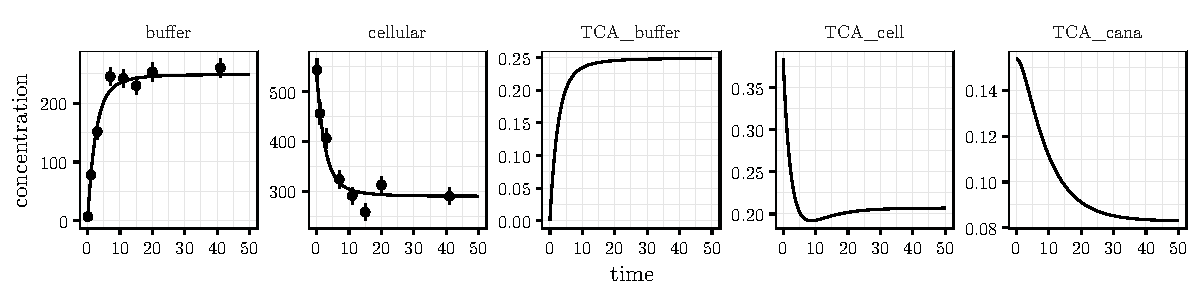
\includegraphics[width = \textwidth]{Figures/figure2}
\caption{Model prediction of the observable and internal states. Simulated data is shown as dots with error bars.\label{fig:observation}}
\end{figure}

\subsection{Parameter transformation}
Parameter transformations play a crucial role in the set-up of \pkg{dMod}. They can have several purposes such as fixing paramer values, implementing parameter bounds, including steady-state constraints or mapping parameters to different conditions. While being conceptually the same, it might be worth noting that parameters can be distinguished in two classes. The first class of parameters are \textit{initial values} for dynamic states, such as \code{TCA_buffer}. Parameters of the second class, such as rate parameters, have no accompanying dynamic state.

First, we use parameter transformations to constrain all parameters to be positive or zero because all our parameters are either amounts or rate parameters. The parameter transformation is generated by the \code{P()} command taking an \code{eqnvec} object. Parameter transformations explicitly state the relation between the \textbf{inner} parameters, i.e., the parameter values that are evaluated within the model, and the \textbf{outer} parameters, i.e., the parameter values provided by the user or by an optimizer. In our case, we imply positivity of inner parameters using the \code{exp()} function on outer parameters.
The corresponding code reads:
\begin{CodeChunk}
\begin{CodeInput}
R> p <- P(
+    trafo = eqnvec(TCA_buffer = "0", TCA_cell = "exp(TCA_cell)",
+      TCA_cana = "exp(TCA_cana)", import = "exp(import)",
+      export_sinus = "exp(export_sinus)", export_cana = "exp(export_cana)",
+      reflux = "exp(reflux)", s = "exp(s)"),
+   condition = "standard")
R> outerpars <- getParameters(p)
R> pouter <- structure(rep(-1, length(outerpars)), names = outerpars)
R> plot((g * x * p)(times, pouter), data)
\end{CodeInput}
\end{CodeChunk}
%
The vector \code{outerpars} is the collection of all symbols on the right-hand side of \code{trafo}. It coincides with \code{names(pars)} except for \code{TCA_buffer}, which is fixed to a constant expression, here 0, by the transformation. However, the interpretation of the parameters has changed since now their values are on a log-scale. All three functions, the observation function, prediction function and parameter transformation can be concatenated to one new prediction function, \code{g * x * p} which takes times and values of the outer parameters to predict internal and observable states. The model prediction generated by \code{pouter} is shown in Figure~\ref{fig:gxp}.

\begin{figure}[t!]
\centering
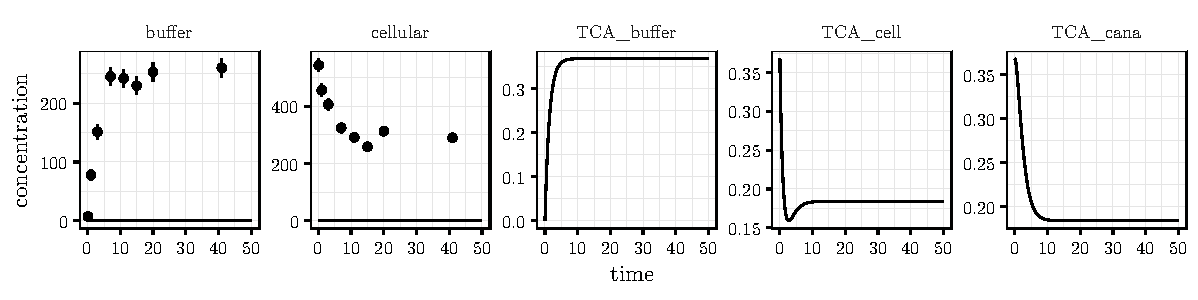
\includegraphics[width = \textwidth]{Figures/figure3}
\caption{Prediction of internal and observed states. All values of the outer parameters have been set to $-1$. Simulated data points are shown as dots with error bars.\label{fig:gxp}}
\end{figure}

\subsection{Objective function and model fitting}
The objective of model fitting is to find parameter values such that the corresponding model prediction matches the observation. In Figure~\ref{fig:gxp}, the graphs of \code{buffer} and \code{cellular} should match the observation within the error.
For normally distributed measurement noise, maxi\-mum-likelihood estimation is equivalent to least-squares estimation. A least-squares objective function can be generated by the \code{normL2()} command which requires a \code{datalist} object, in our case \code{data}, and a prediction function, in our case \code{g * x * p}.

If prior knowledge for parameter values is available, this can be incorporated by calling \code{constraintL2()}. The function penalizes distances between arbitrary prior values and parameter values with a quadratic function weighted by the strength of the prior. Thereby, parameters are treated like observations with normally distributed error. The objective functions returned by \code{normL2()} and \code{constraintL2()} are objects of class \code{objfn} and can be added by the \code{"+"} operator.

Frequently, non-identifiable parameters are encountered in non-linear dynamic systems. In this case, adding a weak prior to all parameters prevents the optimizer from selecting extreme parameter values for which the ODE solver aborts. This situation is to be distinguished from the prior knowledge case. A general prior is only used during model development to facilitate parameter estimation and should be dropped in the end. To distinguish prior knowledge contributions from a general prior in the objective value, the \code{attr.name} argument of \code{constraintL2()} can be used. Numeric attributes from objective functions added by the \code{"+"} operator are collected and values from equally named attributes are added. Setting \code{attr.name = "data"} causes the prior to be combined with the data likelihood whereas \code{attr.name = "prior"} distinguishes it from the data. 

\begin{figure}[t!]
\centering
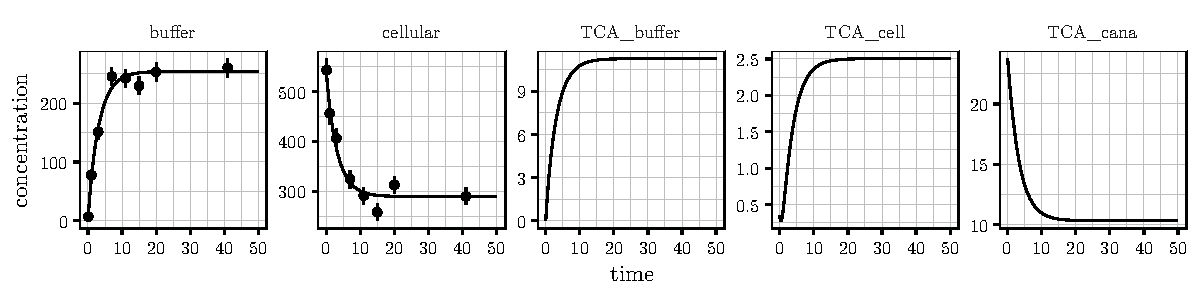
\includegraphics[width = \textwidth]{Figures/figure4}
\caption{Prediction of internal and observed states after optimization of the objective function. Simulated data points are shown as dots with error bars.}
\label{fig:myfit}
\end{figure}

The following code illustrates the implementation of the objective function and how it is used with the \code{trust()} optimizer from the \pkg{trust} package \citep{trust} to obtain a model fit, shown in Figure~\ref{fig:myfit}.
%
\begin{CodeChunk}
\begin{CodeInput}
R> obj <- normL2(data, g * x * p) + constraintL2(pouter, sigma = 10)
R> myfit <- trust(obj, pouter, rinit = 1, rmax = 10)
R> plot((g * x * p)(times, myfit$argument), data)
\end{CodeInput}
\end{CodeChunk}
%
Besides non-identifiability of parameters, local optima constitute another pit-fall when optimizing non-linear functions. The \code{trust()} optimizer employs derivative information and therefore, if starting within a certain region around a local optimum, is very efficient in finding it back. Once an optimum is found, we can be confident that there is no deeper point around. However, to be confident that an optimum is the globally best solution, we might want to scatter starting points for optimization runs all over the parameter space. The \pkg{dMod} package provides the \code{mstrust()} function based on \code{trust()} to do a multi-start search:
%
\begin{CodeChunk}
\begin{CodeInput}
R> out_mstrust <- mstrust(obj, pouter, rinit = 1, rmax = 10, iterlim = 500,
+    sd = 4, cores = 4, fits = 50)
R> myframe <- as.parframe(out_mstrust)
R> plotValues(myframe, tol = 0.01, value < 100)
R> plotPars(myframe, tol = 0.01, value < 100)
\end{CodeInput}
\end{CodeChunk}
Here, we have searched according to $\vec p_i = \vec p_0 + \Delta\vec p_i$ where $\vec p_0$ is the center, in our case \code{pouter}, $\Delta\vec p_i\sim N(0, \sigma^2)$ is a random parameter vector taken from a normal distribution, in our case $\sigma = 4$, and the index $i$ runs from 1 to \code{fits = 50}. The \code{mclapply()} command from the standard \pkg{parallel} package \citep{parallel} is used internally to run fits in parallel, here \code{cores = 4}. The result of \code{mstrust()} is a list of all returned values of \code{trust()}. To extract the final objective value, parameter values, convergence information and the number of iterations, \code{as.parframe()} is used. The multi-start approach identifies four local optima, see Figure~\ref{fig:mstrust}, which yield almost the same objective value, Figure~\ref{fig:mstrust}A.
\begin{figure}[t!]
\centering
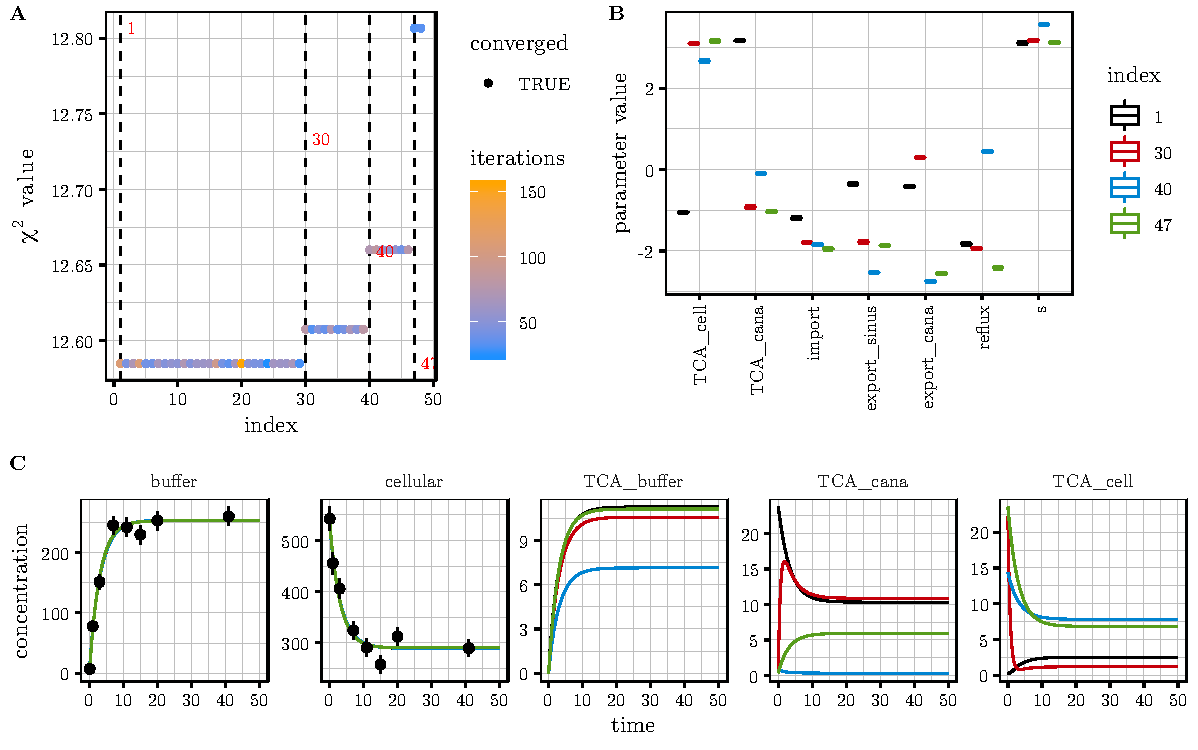
\includegraphics[width = \textwidth]{Figures/figure5}
\caption{Result of multi-start fitting procedure. (A) Fits have been sorted by increasing objective value. Four optima were found with almost identical objective value. (B) The parameter values for different optima are shown in different colors. (C) Each local optimum corresponds to a different model prediction, shown in different colors. The observed states are pracitically undistinguishable although the internal states show different behavior.}
\label{fig:mstrust}
\end{figure}
Despite the similar objective value, the optima are not close to each other in parameter space, as being illustrated by Figure~\ref{fig:mstrust}B, and lead to different predictions, Figure~\ref{fig:mstrust}C. 
Figure~\ref{fig:mstrust}B suggests that the two initial values \code{TCA_cell} and \code{TCA_cana} are connected in the sense that if one takes a large value, the other takes a small value and vice versa.
%From the initial value parameters \code{TCA_cell} and \code{TCA_cana} it seems that they are exchangeable. Where \code{TCA_cell} is high, \code{TCA_cana} is low and vice versa. 
This is not surprising because the observed cellular TCA amount is the sum of both. A new experiment needs to be designed to distinguish one situation from another.


\subsection{Working with several conditions}\label{sec:conditions}
In practice, the canaliculi only form a closed compartment if Ca$^{2+}$/Mg$^{2+}$ ions are present in the buffer. Therefore, if the experiment is repeated with Ca$^{2+}$/Mg$^{2+}$-free efflux buffer, the contents of the canaliculi escapes quickly into the buffer compartment. Under this condition, the \code{buffer} measurement reflects what was formerly the total TCA content in buffer and canaliculi whereas the \code{cellular} measurement reflects what was fomerly the TCA content of the cells.
Mathematically, two experimental conditions which differ only by the \code{reflux} parameter need to be combined in one objective function.

Like before, we simulate a data set. Then, a parameter transformation for the additional condition is set up and the parameter space is explored by a multi-start fit.

To simulate the new experimental condition, the \code{"reflux"} parameter is modified. The new data set is combined with the original data by the \code{"+"} operator.
%
\begin{CodeChunk}
\begin{CodeInput}
R> pars["reflux"] <- 1e3
R> out <- (g*x)(times, pars, conditions = "open")
R> datasheet <- subset(as.data.frame(out),
+    time %in% timesD & name %in% names(observables))
R> datasheet <- within(datasheet, {
+    sigma <- sqrt(value + 1)
+    value <- rnorm(length(value), value, sigma)
+  })
R> data <- data + as.datalist(datasheet)
\end{CodeInput}
\end{CodeChunk}
%
To add a condition to the parameter transformation function, we use the equations of the standard condition as a template for the ``open'' condition. Parameter transformation functions for different conditions are combined by the \code{"+"} operator.
%
\begin{CodeChunk}
\begin{CodeInput}
R> trafo <- getEquations(p, conditions = "standard")
R> trafo["reflux"] <- "exp(reflux_open)"
R> p <- p + P(trafo, condition = "open")
\end{CodeInput}
\end{CodeChunk}
%
Both transformations ``standard'' and ``open'' now possess the outer parameters \code{reflux} and \code{reflux_open}. However, the value of \code{reflux} is mapped to an inner parameter only by transformation ``standard''. Accordingly, transformation ``open'' only uses \code{reflux_open}. 
%Compared to the situation before we have gained the outer parameter \code{reflux_open}. Both transformations, "standard" and "open", evaluate the same vector of outer parameters meaning that they 
Thus, both transformations return the same values for all but the \code{reflux} parameter. The prediction function \code{g * x} is generic in the sense that \code{condition = NULL} whereas the concatenation \code{g * x * p} has the conditions ``standard'' and ``open'', evaluating the identical function \code{g * x} on two parameter vectors.

We define an updated objective function:
\begin{CodeChunk}
\begin{CodeInput}
R> outerpars <- getParameters(p)
R> pouter <- structure(rep(-1, length(outerpars)), names = outerpars)
R> obj <- normL2(data, g * x * p) + constraintL2(pouter, sigma = 10)
\end{CodeInput}
\end{CodeChunk}
%
Then we start 50 fits around \code{pouter}. The list of fits is simplified to a \code{parframe} and by the \code{as.parvec()} function, the parameter vector (of the best fit) is extracted from the \code{parframe}. The best fit is used to make a prediction which is plotted together with the simulated data. All results are shown in Figure~\ref{fig:twoconditions}.
%
\begin{CodeChunk}
\begin{CodeInput}
R> out_mstrust <- mstrust(obj, pouter, rinit = 1, rmax = 10, iterlim = 500,
+    sd = 4, cores = 4, fits = 50)
R> myframe <- as.parframe(out_mstrust)
R> plotValues(myframe, tol = 0.1, value < 100)
R> plotPars(myframe, tol = 0.1, value < 100)
R> bestfit <- as.parvec(myframe)
R> plot((g * x * p)(times, bestfit), data)
\end{CodeInput}
\end{CodeChunk}
%
\begin{figure}[t!]
\centering
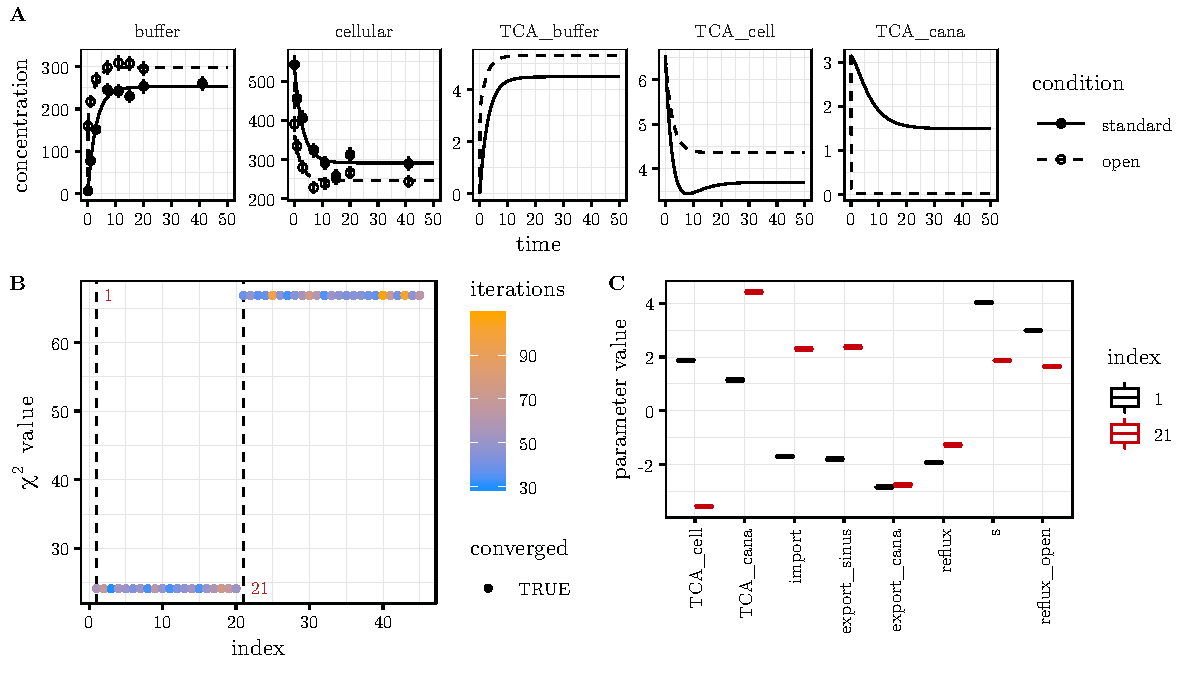
\includegraphics[width = \textwidth]{Figures/figure6}
\caption{Result of multi-start fitting procedure with two experimental conditions. (A) Model prediction of the best fit and the simulated data are shown in different colors. (B) Fits have been sorted by increasing objective value. The lowest value clearly separates from the second plateau. (C) Plotting the parameter values for each of the fits reveals that the second plateau consists of two optima. The lowest plateau however corresponds to a unique optimum.}
\label{fig:twoconditions}
\end{figure}
%
Interestingly, with the new experiment the best optimum becomes unique. The log-likelihood difference, i.e., half the difference between the objective values, is more than 20 between the lowest and the second plateau, which is highly significant. The uniqueness of the lowest plateau is confirmed by Figure~\ref{fig:twoconditions}C which shows no scattering of the black circles.

\subsection{Parameter uncertainty and identifiability}
\label{chap_uncertainty}

One might wonder why the optimum is unique as for any choice of the scaling parameter \code{s} we find appropriate values of the TCA initial value parameters that give rise to exactly the same prediction of the observables. The reason for the uniqueness is the parameter $L_2$-constraint that we have added to the objective function. Nonetheless, we will see, that the non-identifiability is still visible in the profile likelihood.

The profile likelihood is computed by the \code{profile()} command. There are several options to control the step-size and accuracy. For convenience the \code{method} option can be used to select between the presets \code{"integrate"} and \code{"optimize"}.

\begin{figure}[t!]
\centering
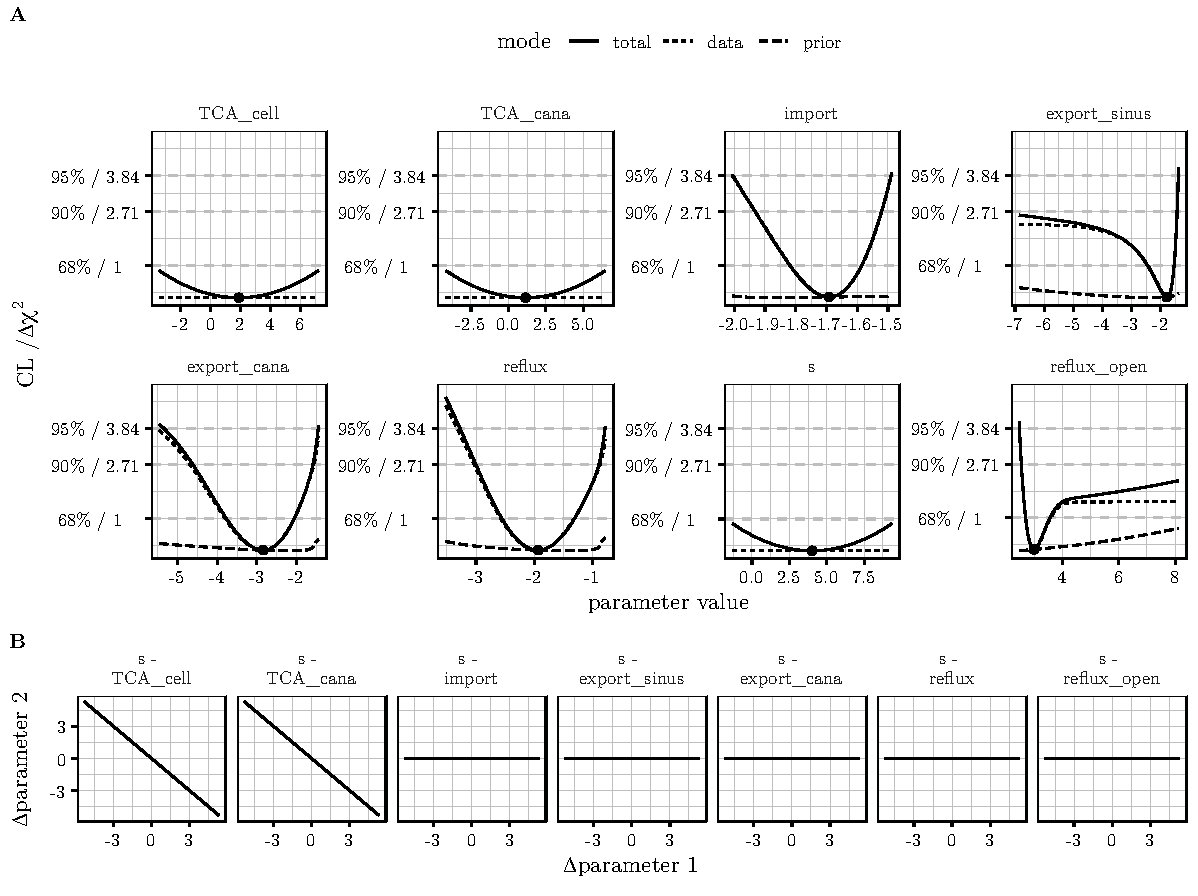
\includegraphics[width = \textwidth]{Figures/figure7}
\caption{Profile likelihood. (A) Profiles of all parameters. Data- and prior contribution to the total objective value are distinguished by line-type. (B) Parameter paths for the scaling parameter \code{s}.\label{fig:pl}}
\end{figure}

The code
\begin{CodeChunk}
\begin{CodeInput}
R> profiles <- profile(obj, bestfit, names(bestfit), limits = c(-5, 5),
+    cores = 4)
R> plotProfile(profiles)
R> plotPaths(profiles, whichPar = "s")
\end{CodeInput}
\end{CodeChunk}
%
gives us the result shown in Figure~\ref{fig:pl}.
Computing the profile likelihood, the sum of data contribution, \code{normL2}, and prior contribution, \code{constraintL2}, are optimized under the constraint of a given parameter value for the profiled parameter. In the optimum, data and prior contribution are evaluated separately giving rise to the dashed and dotted lines in Figure~\ref{fig:pl}A. As we had expected, the data contribution to the initial value parameters \code{TCA_cell}, \code{TCA_cana} and the scaling parameter \code{s} is constantly zero. The parameters are structurally non-identifiable.

Each profile corresponds to a certain path in parameter space. The path for the profile of the non-identifiable scaling parameter \code{s} is shown in Figure~\ref{fig:pl}B. It shows a clear coupling of the scaling parameter \code{s} and the initial value parameters \code{TCA_cell} and \code{TCA_cana}: both initial value parameters have to be decreased by the same extent as the scaling parameter is increased to keep the prediction unchanged.

The profiles of the parameters \code{export_sinus} and \code{reflux_open} exceed the 95\% confidence threshold only to one side. Given the data, the \code{export_sinus} parameter could equally be $-\infty$ (corresponding to an export rate of 0) without changing the likelihood significantly for the worse. A similar statement holds for the \code{reflux_open} parameter which could equally be $\infty$ meaning that we could assume instantaneous draining of the canaliculi for the \code{"open"} condition. The two parameters are practically non-identifiable.

Finally, the parameters \code{import}, \code{export_cana} and \code{reflux} exceed the 95\% confidence threshold in both directions meaning that the parameters have finite confidence intervals. However, the confidence intervals are rather large and we might ask if there is further information that we could use to improve parameter identifiability without generating new data.

\subsection{Steady-state constraints and implicit transformations}
\label{chap_steady_state}

So far we have estimated both initial concentrations, \code{TCA_cell} and \code{TCA_cana}, independently. However, we know that the efflux experiment was just started after completion of the uptake process. Our system runs into a steady state, the buffer is exchanged and the measurement begins. Hence, we can use the steady-state condition as an additional information for the modeling process.

The steady-state relation between \code{TCA_cana} and \code{TCA_cell} can be derived analytically from the ODE, Figure~\ref{fig:flowchart}A, by setting the right-hand side of $\frac{\rm d}{ {\rm d}t} \verb!TCA_cana!$ to zero. It reads
%
\begin{equation}
\verb!TCA_cana! = \verb!export_cana * TCA_cell / reflux!
\label{}
\end{equation}
%
This relation can be explicitly used in a parameter transformation to express \code{TCA_cana} in terms of other parameters. The dimension of the parameter space is thereby reduced by one. The following implementation shows how we would use the existing transformation function \code{p} to generate an alternative transformation function \code{pSS} which includes the steady-state condition and replaces \code{p} in the prediction function \code{g * x * p}.
%
\begin{CodeChunk}
\begin{CodeInput}
R> pSS <- NULL
R> equations <- getEquations(p)
R> conditions <- names(equations)
R> for (n in conditions) {
+    equations[[n]]["TCA_cana"] <- "exp(export_cana)*exp(TCA_cell)/exp(reflux)"
+    pSS <- pSS + P(equations[[n]], condition = n)
+  }
\end{CodeInput}
\end{CodeChunk}
%
We get all the information about the transformations from the \code{getEquations()} command. The equation for \code{TCA_cana} is substituted by our steady-state constraint. By the \code{"+"} operator, a new parameter transformation function \code{pSS} is iteratively constructed for all conditions.

Alternatively, we want to implement the steady-state constraint by an \textit{implicit} parameter transformation, as opposed to the explicit transformation shown above. Let $\dot x = f(x, p)$ be our dynamic system. Then, under certain conditions, we find a function $g(p)$ such that $f\big( g(p), p\big) = 0$ for all $p$, i.e., $x_S = g(p)$ is a steady state of $f$. The parameter transformation we want to generate is the function $p \mapsto \big(p, g(p)\big)$. Here, the set of outer parameters is the set of the reaction rates  $p$ whereas the set of inner parameters contains these rates and the corresponding steady states as initial value parameters. The root of $f$ must be determined numerically to which end \code{multiroot()} from the \pkg{rootSolve} package \citep{rootSolve} is used.

The following code is a reimplementation of the example above. The replacement of the buffer and the possibility for different reflux rates between the ``standard'' and  ``open'' conditions are explicitly modeled by events at time zero. 
%
\begin{CodeChunk}
\begin{CodeInput}
R> reactions <- NULL
R> reactions <- addReaction(reactions, "TCA_buffer", "TCA_cell",
+    rate = "import*TCA_buffer", description = "Uptake")
R> reactions <- addReaction(reactions, "TCA_cell", "TCA_buffer",
+    rate = "export_sinus*TCA_cell", description = "Sinusoidal export")
R> reactions <- addReaction(reactions, "TCA_cell", "TCA_cana",
+    rate = "export_cana*TCA_cell", description = "Canalicular export")
R> reactions <- addReaction(reactions, "TCA_cana", "TCA_buffer",
+    rate = "(reflux*(1-switch) + reflux_open*switch)*TCA_cana",
+    description = "Reflux into the buffer")
R> reactions <- addReaction(reactions, "0", "switch", rate = "0",
+    description = "Create a switch")
\end{CodeInput}
\end{CodeChunk}
%
The events for \code{TCA_buffer} and \code{switch} are generated as part of the model and, therefore, need to be provided to the \code{odemodel()} command together with the model.
%
\begin{CodeChunk}
\begin{CodeInput}
R> events <- NULL
R> events <- addEvent(events, var = "TCA_buffer", time = 0, value = 0      )
R> events <- addEvent(events, var = "switch"    , time = 0, value = "OnOff")
R> mymodel <- odemodel(reactions, modelname = "bamodel2", events = events)
R> x <- Xs(mymodel)
\end{CodeInput}
\end{CodeChunk}
%
Event times and values can both be either numeric or a character representing a parameter. These parameters are treated in the same way as all other parameters, meaning that they can be set in a condition-specific way or be estimated.

For the implicit parameter transformation we need the ODE which is obtained by the command \code{as.eqnvec()} from the reactions. The Jacobian of $f$ is rank-deficient because the system has a conserved quantity $c = \verb!TCA_buffer + TCA_cana + TCA_cell!$ which is the total TCA amount. Replacing one element of $f$ by $c - \verb!TCA_tot!$, the rank of the Jacobian is completed, the condition for the local existence of the implicit function $g(p)$ is satisfied and the steady state is parameterized by $p$ and the additional parameter \code{TCA_tot}.
%
\begin{CodeChunk}
\begin{CodeInput}
R> f <- as.eqnvec(reactions)[c("TCA_buffer", "TCA_cana", "TCA_cell")]
R> f["TCA_cell"] <- "TCA_buffer + TCA_cana + TCA_cell - TCA_tot"
R> pSS <- P(f, method = "implicit", compile = TRUE, modelname = "pfn")
\end{CodeInput}
\end{CodeChunk}
%
For the optimization, all outer parameters should still be log-parameters, implemented by an explicit parameter transformation. Outer parameters for the initial values are not necessary any more. They can be replaced by 0 since the initial values are computed by the implicit transformation. The switch parameter \code{OnOff} is defined in a condition-specific way: zero for the ``standard'' condition and one for the ``open'' condition. The final transformation will be a concatenation of the implicit and explicit transformations: \code{pSS*p}.
%
\begin{CodeChunk}
\begin{CodeInput}
R> innerpars <- unique(c(getParameters(mymodel), getSymbols(observables),
+    getSymbols(f)))
R> trafo <- repar("x~x"     , x = innerpars)
R> trafo <- repar("x~0"     , x = reactions$states, trafo)
R> trafo <- repar("x~exp(x)", x = setdiff(innerpars, "OnOff"), trafo)
R> p <- P(repar("OnOff~0", trafo), condition = "standard") +
+    P(repar("OnOff~1", trafo), condition = "open")
\end{CodeInput}
\end{CodeChunk}
%
Although the observables have not changed compared to the set-up with purely explicit transformations, the observation function must be generated again because the ODEs have structurally changed and a new parameter \code{reflux_open} has appeared. Using the old observation function would result in a wrong propagation of parameter sensitivities.
%
\begin{CodeChunk}
\begin{CodeInput}
R> g <- Y(observables, f = x, compile = TRUE, modelname = "obsfn2")
\end{CodeInput}
\end{CodeChunk}
%
Finally, the objective function is defined. The prediction function is now a concatenation of four functions.
%
\begin{CodeChunk}
\begin{CodeInput}
R> outerpars <- getParameters(p)
R> pouter <- structure(rep(-1, length(outerpars)), names = outerpars)
R> obj <- normL2(data, g * x * pSS * p) + constraintL2(pouter, sigma = 10)
\end{CodeInput}
\end{CodeChunk}
%
The same simulated data set has been fitted by the fully explicit and the implicit/explicit model implementations. In both cases the global optimum is unique. Parameter profiles have been computed with both model implementations, shown in Figure~\ref{fig:allprofiles}. In addition, the original profiles without steady-state constraints are plotted.
%
\begin{figure}[t!]
\centering
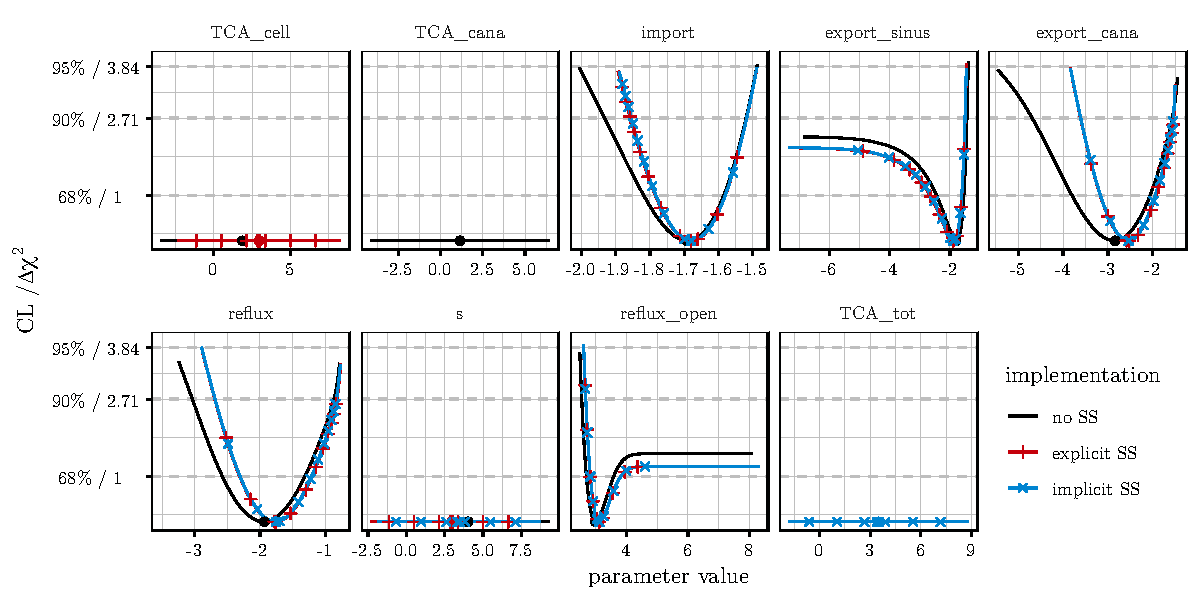
\includegraphics[width = \textwidth]{Figures/figure8}
\caption{Parameter profiles for three different model implementations. The profile likelihood around the global optimum for the models without steady-state constraints, explicit steady-state constraints and implicit implementation of steady states is visualized by different colors. To illustrate that explicit (red) and implicit (blue) steady-state implementations yield the same result, the corresponding profiles are highlighted by red plus and blue cross signs, respectively.
\label{fig:allprofiles}}
\end{figure}
%
The optima found by all three approaches, no steady-state, analytic steady-state and numeric steady-state, are statistically compatible. The two implementations using the steady-state information show exactly the same profiles. Since one formulation is parameterized by \code{TCA_cell} whereas the other is parameterized by \code{TCA_tot}, the plot highlights one of the fundamental properties of the profile likelihood: invariance under reparameterization. In comparison to the profiles without steady-state information, the new profiles are narrower, meaning that the parameters have smaller confidence intervals. This was to be expected because we have reduced the dimension of the parameter space by one.

\subsection{Prediction uncertainty and validation profiles}

Combining the steady-state constraint and two efflux experiments, one with
closed canaliculi and the other with open canaliculi, we could fully identify
the rate parameters \code{import}, \code{export_cana} and \code{reflux}. The
amount parameter \code{TCA_tot} is fully coupled with the scaling parameter
\code{s} such that both are structurally non-identifiable. The parameters
\code{export_sinus} and \code{reflux_open} are practically non-identifiable
since both parameters cannot be constrained to a finite interval with 95\%
confidence.

Next, we investigate the possibility to predict cellular amounts of TCA,
\code{TCA\_cell}, despite the non-identifiability of parameters. 
The amount of \code{TCA\_cell} certainly depends on the total
amount of TCA in the system. This total amount must be fixed in which case the
parameters \code{TCA\_cell}, \code{TCA\_cana} and \code{s} become identifiable.
The prediction uncertainty is assessed by a \textit{prediction profile}
which is computed based on a virtual data point for cellular TCA, measured at
time point $t = 41$ in the ``standard'' condition. The \pkg{dMod} formulation reads as:
%
\begin{CodeChunk}
\begin{CodeInput}
R> obj.validation <- datapointL2(name = "TCA_cell", time = 41, value = "d1",
+    sigma = 0.002, condition = "standard")
\end{CodeInput}
\end{CodeChunk}
%
The uncertainty $\sigma = 0.002$ is set to a small
value, i.e., below 1\% of the prediction value. The \code{datapointL2()}
command returns an objective function which evaluates the model prediction\footnote{Several objective functions combined by the \code{"+"} operator
share the same environment. Thus, the prediction computed by the first
objective function can be evaluated by all other functions to come.} and
computes the least-squares function of the virtual datapoint, returning
derivatives for the data-point parameter \code{d1}. Its value ``d1'' is yet to be
determined. By fitting the objective function \code{obj} together with
\code{obj.validation}, ``d1'' equals the value of \code{TCA\_cell} at
$t=41$, as only then its contribution to the objective value is zero.
\begin{CodeChunk}
\begin{CodeInput}
R> fixed <- c(TCA_tot = log(1))
R> myfit <- trust(obj + obj.validation,
+    parinit = c(d1 = 1, pouter[!names(pouter) %in% names(fixed)]),
+    fixed = fixed, rinit = 1, rmax = 10)
\end{CodeInput}
\end{CodeChunk}
Using the derivative information provided by \code{datapointL2}, a
prediction profile around \code{d1} is calculated.
\begin{CodeChunk}
\begin{CodeInput}
R> profile_prediction <- profile(obj + obj.validation,
+    myfit$argument, "d1", limits = c(-5, 5), fixed = fixed)
\end{CodeInput}
\end{CodeChunk}
%
The result is shown in Figure~\ref{fig:validation}A. The interpretation of
such a prediction profile is, that a measurement yielding a value for the
cellular TCA level at time point $t=41$ outside of the interval $[0.19,0.21]$
does not conform to our model with 95\% confidence.

\begin{figure}[t!]
\centering
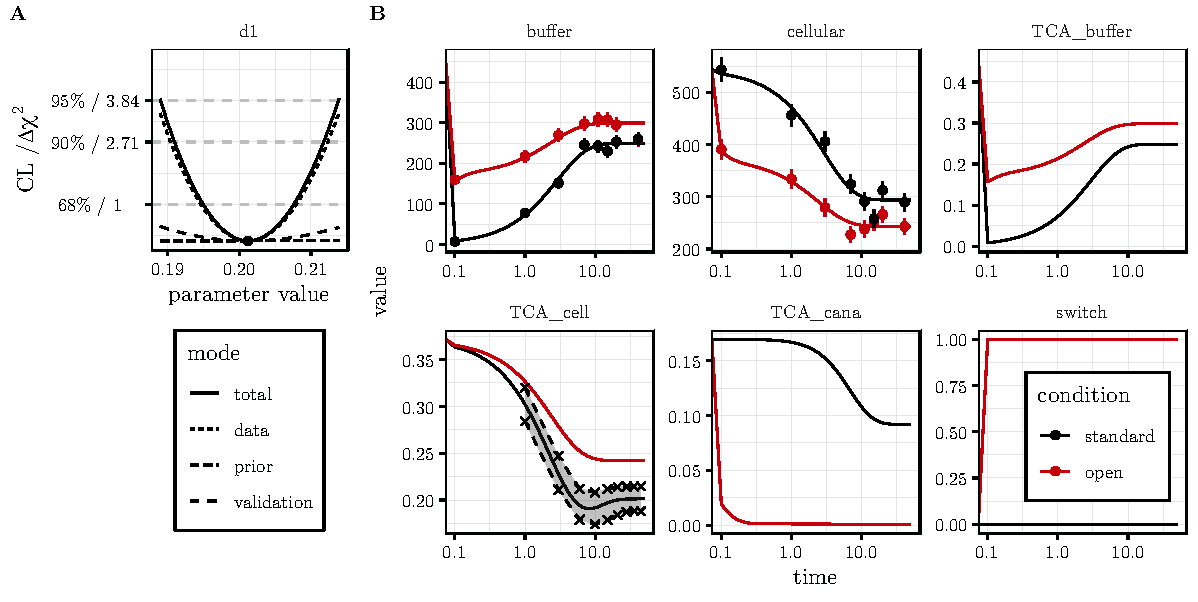
\includegraphics[width = \textwidth]{Figures/figure9}
\caption{Validation profile and confidence bands for the model prediction.
(A) The profile likelihood for the data point parameter \code{d1} describing
\code{TCA\_cell} at time point $t = 41$ is shown. (B) Computing the data
parameter profile for different time points yields 95\% confidence bands on the
prediction of \code{TCA\_cell}.
\label{fig:validation}}
\end{figure}

More precisely, changing the data-point parameter \code{d1}, the model is quickly forced to
match the new data point. This is apparent from the least squares contribution entitled ``validation'' of the virtual data point, returned by \code{obj.validation}. 
The contribution is shown as dashed line in Figure~\ref{fig:validation}A. It remains small at the expense of a larger deviation from original data points, indicated by the ``data'' contribution. 
Forcing \code{d1} and thereby the model
prediction to deviate more than $0.01$ from the original value, the profile
exceeds the 95\% confidence threshold providing a confidence interval for the
prediction itself. By calculating
prediction profiles for several time points, a confidence band for the course of
\code{TCA\_cell} is constructed as shown in Figure~\ref{fig:validation}B. The
95\% confidence band is closed towards small and large amounts.

In summary, we find that the prediction of cellular TCA amounts is highly
precise despite the non-identifiability of the \code{export_sinus} and
\code{reflux_open} parameters.

\subsection{Speed comparison}

Last but not least, the computational efficiency of \pkg{dMod} was tested. In comparison to other \proglang{R} packages offering functions to estimate parameters of ODE models from experimental data, see Table~\ref{tab:comparison}, \pkg{dMod} provides all observation-, prediction- and parameter transformation functions with derivatives. Those are based on symbolic expressions being translated into \proglang{C} code and being compiled alongside the model itself.

For the comparison, we have tested three different scenarios with \pkg{dMod}. The scenarios approximate the conditions found in different frameworks: (1) The default settings with derivatives and trust region optimization, (2) derivative-free optimization with the Nelder-Mead algorithm and, (3) optimization with the L-BFGS-B algorithm with numerically computed gradient. With either of these settings, the example model has been fitted 50 times and the runtime of each fit has been evaluated. The result of the runtime evaluation is shown in Figure~\ref{fig:comparison} as black dots and violin lines. Since in \pkg{dMod} the ODE model and observation function are compiled, runtime values for the corresponding scenarios with native \proglang{R} code have been roughly estimated to exceed the runtime of compile code by a factor of 50, as indicated by \cite{deSolve}. The extrapolated runtimes are shown in orange. Finally, the available packages for parameter estimation in ODE models have been assigned to one or more scenarios depending on whether the framework supports compiled code or supports sensitivity equations. Except for the runtime values obtained with \pkg{dMod}, these assignments reflects a rough estimate, indicated by an asterisk.  

\begin{figure}[t!]
\centering
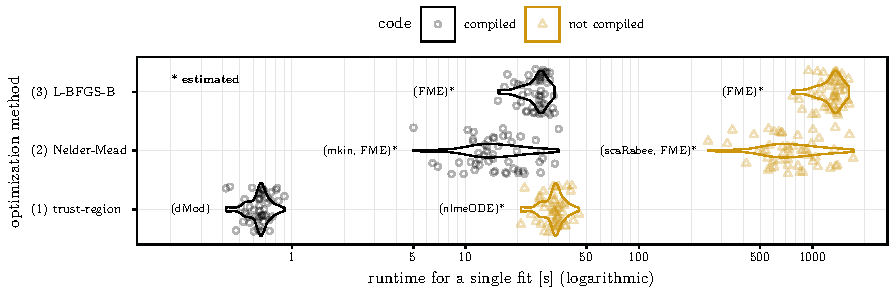
\includegraphics[width=6in]{Figures/figure10}
\caption{Comparison of the runtime for parameter estimation for different scenarios. The runtime values obtained from 50 fits per scenario with \pkg{dMod} are shown as black dots and violin lines. Runtime values for native \proglang{R} code (not compiled) were assumed be 50 times larger, shown as orange triangles and violin lines. Modeling frameworks have been assigned to either of the scenarios based on their characteristics.
\label{fig:comparison}}
\end{figure}

The speed comparison shows that by a combination of compiled code and symbolically derived gradient and hessian, the runtime achieves its best value. The reason for the good performance is that the evaluation of sensitivity equations is only slower by a factor 2-3. On the other hand, the objective function needs to be called only once per iteration of the optimizer whereas the numeric evaluation of the gradient requires many function calls. 

\section[Extensions of dMod]{Extensions of \pkg{dMod}}
\label{sec:extensions}
Computer algebra and symbolic tools are not part of \proglang{R}'s core functionality. In this section we illustrate two symbolic tools that are shiped with \pkg{dMod},  dealing with structural non-identifiability and steady-state constraints. They are implemented in \proglang{Python} and are interfaced via the \pkg{rPython} package \citep{rPython}.

\subsection{Lie-group symmetry detection}
In Section \ref{chap_uncertainty}, profile likelihood computation showed the existence of both practically and structurally non-identifiable parameters. While practical non-identifiability arises from insufficient information in the data, structural non-identifiabilty is connected to Lie-group symmetries, i.e., transformations of the states and parameters \[\Psi: (x,\theta) \longmapsto (x^*, \theta^*)\] that preserve the model prediction of the observables: \[g(x^*, \theta^*) = g(x,\theta)\,.\] Based on \cite{merkt2015higher}, the \code{symmetryDetection()} command outputs a list of available symmetry transformations. For example, the code
%
\begin{CodeChunk}
\begin{CodeInput}
R> reactions <- NULL
R> reactions <- addReaction(reactions, "TCA_buffer", "TCA_cell", 
+    rate = "import_baso*TCA_buffer")
R> reactions <- addReaction(reactions, "TCA_cell", "TCA_buffer", 
+    rate = "export_sinus*TCA_cell")
R> reactions <- addReaction(reactions, "TCA_cell", "TCA_cana", 
+    rate = "export_cana*TCA_cell")
R> reactions <- addReaction(reactions, "TCA_cana", "TCA_buffer", 
+    rate = "reflux*TCA_cana")
R> observables <- eqnvec(buffer = "s*TCA_buffer",
+    cellular = "s*(TCA_cana + TCA_cell)")
R> symmetryDetection(as.eqnvec(reactions), observables)
\end{CodeInput}
\end{CodeChunk}
%
returns the following output:
%
\begin{CodeChunk}
\begin{CodeOutput}
1 transformation(s) found:
variable   : infinitesimal : transformation
-----------------------------------------------------
#1: Type: scaling
TCA_buffer : -TCA_buffer   : TCA_buffer*exp(-epsilon)
TCA_cana   : -TCA_cana     : TCA_cana*exp(-epsilon)
TCA_cell   : -TCA_cell     : TCA_cell*exp(-epsilon)
s	   : s  	   : s*exp(epsilon)
\end{CodeOutput}
\end{CodeChunk}
%
In agreement with the identifiability analysis by the profile-likelihood method, the parameters \code{s}, \code{TCA_buffer}, \code{TCA_cana} and \code{TCA_cell} are found to be non-identifiable due to a scaling symmetry. The corresponding scaling transformation, last column, leaves the observation invariant for any choice of \code{epsilon}. The parameter non-identifiability can be resolved choosing one representative from the orbit of the transformation. In our case, the scaling parameter could, for example, be fixed to 1. 

\subsection{Analytical steady-state constraints}
While for the the present model, the steady-state could be explicitly calculated by hand, this might be much more challenging for models with a large number of states and parameters. For many of these models, the \code{steadyStates()} command outputs an analytical steady-state solution that can be incorporated in the model as an additional parameter transformation. Based on \cite{rosenblatt2016customized}, the steady-state constraint is solved for a combination of state variables and kinetic parameters while positivity of the solution is ensured. As the paper states, the approach outperforms common methods of steady-state implementation with respect to reliability and performance of the optimization process. For our example, the code reads
\begin{CodeChunk}
\begin{CodeInput}
R> steadyStates(reactions, file = "SS.Rds")
\end{CodeInput}
\end{CodeChunk}
%
yielding the output
%
\begin{CodeChunk}
\begin{CodeOutput}
TCA_cana   = TCA_buffer*export_cana*import_baso/(reflux*(export_cana + 
	   export_sinus))
TCA_cell   = TCA_buffer*import_baso/(export_cana + export_sinus)
TCA_buffer = TCA_buffer
\end{CodeOutput}
\end{CodeChunk}
%
The solution is stored in an Rds file. After loading the file by \code{readRDS()}, the equations can be used when defining the parameter transformation.



\bibliography{mybib}{}

\end{document}
